
\documentclass{article}

% if you need to pass options to natbib, use, e.g.:
    \PassOptionsToPackage{numbers}{natbib}
% before loading neurips_2026

% The authors should use one of these tracks.
% Before accepting by the NeurIPS conference, select one of the options below.
% 0. "default" for submission
% \usepackage{neurips_2026}
\usepackage[main, nonanonymous]{neurips_2026}
% Suppress the NeurIPS submission notice at the bottom of the first page.
\makeatletter
\renewcommand{\@notice}{}
\makeatother
\AtBeginDocument{\nolinenumbers}
% the "default" option is equal to the "main" option, which is used for the Main Track with double-blind reviewing.
% 1. "main" option is used for the Main Track
%  \usepackage[main]{neurips_2026}
% 2. "position" option is used for the Position Paper Track
%  \usepackage[position]{neurips_2026}
% 3. "eandd" option is used for the Evaluations & Datasets Track
 % \usepackage[eandd]{neurips_2026}
 % if you need to opt-in for a single-blind submission in the E&D track:
 %\usepackage[eandd, nonanonymous]{neurips_2026}
% 4. "creativeai" option is used for the Creative AI Track
%  \usepackage[creativeai]{neurips_2026}
% 5. "sglblindworkshop" option is used for the Workshop with single-blind reviewing
 % \usepackage[sglblindworkshop]{neurips_2026}
% 6. "dblblindworkshop" option is used for the Workshop with double-blind reviewing
%  \usepackage[dblblindworkshop]{neurips_2026}

% After being accepted, the authors should add "final" behind the track to compile a camera-ready version.
% 1. Main Track
 % \usepackage[main, final]{neurips_2026}
% 2. Position Paper Track
%  \usepackage[position, final]{neurips_2026}
% 3. Evaluations & Datasets Track
 % \usepackage[eandd, final]{neurips_2026}
% 4. Creative AI Track
%  \usepackage[creativeai, final]{neurips_2026}
% 5. Workshop with single-blind reviewing
%  \usepackage[sglblindworkshop, final]{neurips_2026}
% 6. Workshop with double-blind reviewing
%  \usepackage[dblblindworkshop, final]{neurips_2026}
% Note. For the workshop paper template, both \title{} and \workshoptitle{} are required, with the former indicating the paper title shown in the title and the latter indicating the workshop title displayed in the footnote.
% For workshops (5., 6.), the authors should add the name of the workshop, "\workshoptitle" command is used to set the workshop title.
% \workshoptitle{WORKSHOP TITLE}

% "preprint" option is used for arXiv or other preprint submissions
 % \usepackage[preprint]{neurips_2026}

% to avoid loading the natbib package, add option nonatbib:
%    \usepackage[nonatbib]{neurips_2026}

\usepackage{times}
\usepackage{latexsym}
\usepackage{graphicx}
\usepackage{subcaption} % 必须引入这个包
% For proper rendering and hyphenation of words containing Latin characters (including in bib files)
\usepackage[T1]{fontenc}
\usepackage{multirow}
% For Vietnamese characters
% \usepackage[T5]{fontenc}
% See https://www.latex-project.org/help/documentation/encguide.pdf for other character sets

% This assumes your files are encoded as UTF8
\usepackage[utf8]{inputenc}
\usepackage{booktabs}
\usepackage{siunitx} % 用于数字对齐（可选）
% This is not strictly necessary, and may be commented out,
% but it will improve the layout of the manuscript,
% and will typically save some space.
\usepackage{microtype}

% This is also not strictly necessary, and may be commented out.
% However, it will improve the aesthetics of text in
% the typewriter font.
\usepackage{inconsolata}
\usepackage{booktabs}  % 提供 \toprule, \midrule, \bottomrule，是学术表格的灵魂
\usepackage{array}     % 增强表格列格式控制
\usepackage[table]{xcolor} % 提供 \rowcolor，用于给行添加底纹（高级感的来源）
\usepackage{wrapfig}

%Including images in your LaTeX document requires adding
%additional package(s)
\usepackage{graphicx}
\usepackage{tabularx}
\usepackage{booktabs}
\usepackage{multirow}
\usepackage{graphicx}
\usepackage{amsmath}

\usepackage{pgfplots}
\pgfplotsset{compat=1.18}


% --- 定义高级感配色 ---
\definecolor{myblue}{RGB}{79, 129, 189}    % 沉稳蓝 (B* = n)
\definecolor{myorange}{RGB}{192, 80, 77}   % 莫兰迪红/砖红 (B* != n)
\definecolor{gridgray}{RGB}{220, 220, 220} % 浅灰色网格

\usepackage[utf8]{inputenc} % allow utf-8 input
\usepackage[T1]{fontenc}    % use 8-bit T1 fonts
\usepackage{hyperref}       % hyperlinks
\hypersetup{
    colorlinks=true,
    citecolor=[rgb]{0, 0.4, 0.7}, % 比较深邃的蓝色，类似很多顶会论文的风格
    linkcolor=red,               % 图表引用颜色
    urlcolor=blue                % 网页链接颜色
}
\usepackage{url}            % simple URL typesetting
\usepackage{booktabs}       % professional-quality tables
\usepackage{amsfonts}       % blackboard math symbols
\usepackage{nicefrac}       % compact symbols for 1/2, etc.
\usepackage{microtype}      % microtypography
\usepackage{xcolor}         % colors

\usepackage{enumitem}

% Note. For the workshop paper template, both \title{} and \workshoptitle{} are required, with the former indicating the paper title shown in the title and the latter indicating the workshop title displayed in the footnote. 
% \title{Beyond Static Parallelism: Instance-Adaptive Block Sizing for Diffusion-Based Speculative Decoding}
% \title{Decoding as Policy: Instance-Adaptive Decoding Policy Learning for Diffusion-based Speculative Decoding}
\title{BlockPilot: Instance-Adaptive Policy Learning for Diffusion-based Speculative Decoding}


% The \author macro works with any number of authors. There are two commands
% used to separate the names and addresses of multiple authors: \And and \AND.
%
% Using \And between authors leaves it to LaTeX to determine where to break the
% lines. Using \AND forces a line break at that point. So, if LaTeX puts 3 of 4
% authors names on the first line, and the last on the second line, try using
% \AND instead of \And before the third author name.

\author{
    Hao Zhang \quad Yiming Hu\footnotemark[2] \quad Yong Wang\footnotemark[2] \hspace{0.8em} 
    Mingqiao Mo \quad Xin Xiao \quad Xiangxiang Chu \\[1.2ex]
    AMAP, Alibaba Group \\
    \normalsize\href{https://github.com/AMAP-ML/BlockPilot}{https://github.com/AMAP-ML/BlockPilot}
}

% \author{%
%   David S.~Hippocampus\thanks{Use footnote for providing further information
%     about author (webpage, alternative address)---\emph{not} for acknowledging
%     funding agencies.} \\
%   Department of Computer Science\\
%   Cranberry-Lemon University\\
%   Pittsburgh, PA 15213 \\
%   \texttt{hippo@cs.cranberry-lemon.edu} \\
%   % examples of more authors
%   % \And
%   % Coauthor \\
%   % Affiliation \\
%   % Address \\
%   % \texttt{email} \\
%   % \AND
%   % Coauthor \\
%   % Affiliation \\
%   % Address \\
%   % \texttt{email} \\
%   % \And
%   % Coauthor \\
%   % Affiliation \\
%   % Address \\
%   % \texttt{email} \\
%   % \And
%   % Coauthor \\
%   % Affiliation \\
%   % Address \\
%   % \texttt{email} \\
% }


\begin{document}


\maketitle


\begin{abstract}
Speculative decoding accelerates inference by using a lightweight draft model to generate candidate tokens in parallel, and are then verified by the target model, enabling lossless acceleration. Recently, diffusion-based speculative decoding further improves parallelism by generating multiple tokens per forward pass via block-level diffusion, achieving state-of-the-art (SOTA) performance. However, existing methods adopt a fixed inference block size and assume a uniform optimal decoding strategy across all inputs. In this paper, we show that this assumption is suboptimal, as the optimal block size varies across samples and plays a critical role in speculative decoding performance. Moreover, these values exhibit a clear local structure, concentrating around the training block size, which reduces the problem to a low-dimensional and structured decision space. Based on these insights, we propose BlockPilot, a sample-adaptive policy that predicts the optimal block size from the prefilling representation. Specifically, we formulate block size selection as a lightweight policy learning problem and propose an instance-adaptive decision mechanism that predicts the optimal block size based on the representation of the prefilling stage. The prediction is performed only once after prefilling, allowing for seamless integration. Extensive experiments demonstrate that our method is plug-and-play, introduces minimal overhead, and consistently improves efficiency, achieving an acceptance length of 5.92 and a 4.20$\times$ speedup on Qwen3-4B under temperature $T=1$.

{
\renewcommand{\thefootnote}{\fnsymbol{footnote}}
\footnotetext[2]{\ Project lead and corresponding author.}
}

\end{abstract}


\section{Introduction}
\begin{wrapfigure}{r}{0.46\textwidth}
\vspace{-10pt}
\centering
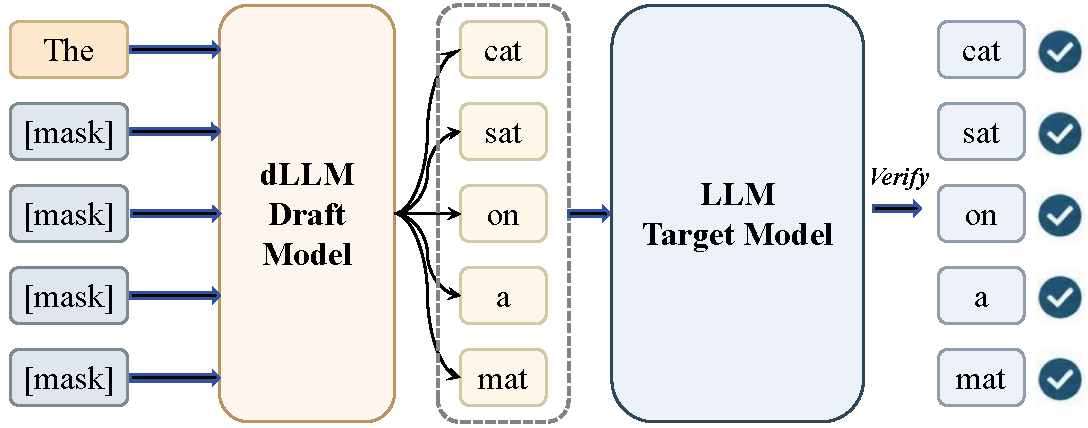
\includegraphics[width=0.46\textwidth]{IMG/Figure1.pdf}
\vspace{-8pt}
\caption{Diffusion-based speculative decoding with a dLLM draft model. The dLLM proposes a block of tokens in parallel, while the target LLM verifies the block and accepts the longest consistent prefix.}
\label{fig:sp}
\vspace{-10pt}
\end{wrapfigure}

Large Language Models (LLMs) \cite{touvron2023open,yang2025qwen3,chiang2023vicuna} have achieved remarkable performance across a wide range of tasks \citep{annepaka2025large,hadi2023large}, demonstrating strong capabilities in reasoning, code generation, and open-ended dialogue. Despite these advances, their inference efficiency is still fundamentally constrained by token-by-token autoregressive decoding \cite{tay2022efficient,papa2024survey,wan2023efficient}. Since each token must be generated conditioned on previously produced tokens, the decoding process is inherently sequential, leading to high latency and limited parallelism, especially for long-form generation. To alleviate this bottleneck, speculative decoding \cite{leviathan2023fastinferencetransformersspeculative, li2025eaglespeculativesamplingrequires, li2024eagle2fasterinferencelanguage, li2025eagle3scalinginferenceacceleration, cai2024medusasimplellminference} introduces a lightweight draft model to propose multiple candidate tokens ahead of the target model. These candidates are then verified by the target model in parallel, allowing multiple tokens to be accepted within a single decoding step. As a result, speculative decoding enables lossless acceleration without altering the output distribution of the target model.


% \begin{figure}[t]
%     \centering
%     \includegraphics[width=0.48\textwidth]{IMG/sp_cropped.pdf}
%     \caption{Speculative decoding paradigm using a diffusion-based draft model (dLLM). Starting from a prefix token (``The''), the draft model generates multiple tokens in parallel via a single denoising step, forming a block of size $B=5$ with four masked positions. The target autoregressive LLM subsequently verifies the proposed tokens, accepting the longest consistent prefix while discarding mismatched predictions.}
%     \label{fig:sp}
% \end{figure}


In recent years, diffusion-based language models (dLLMs) \cite{nie2025largelanguagediffusionmodels, arriola2025blockdiffusioninterpolatingautoregressive, wu2025fastdllmv2efficientblockdiffusion, cheng2025sdarsynergisticdiffusionautoregressionparadigm} have emerged as a promising direction, and diffusion-driven speculative decoding further improves parallelism. By using a dLLM as the draft model, block-wise diffusion enables the generation of multiple tokens in a single forward pass, significantly reducing decoding latency and improving hardware utilization. Fig.~\ref{fig:sp} illustrates the paradigm of speculative decoding based on diffusion models. However, early approaches \cite{li2025diffuspecunlockingdiffusionlanguage,sandler2025specdiff2scalingdiffusiondrafter,samragh2025llmknowsfutureuncovering} rely on large diffusion models and exhibit weak coupling with the target model, limiting their practicality. More recently, DFlash~\cite{chen2026dflash} achieves the first practically deployable state-of-the-art (SOTA) performance in block diffusion-based speculative decoding. By injecting hidden representations from the target model into the diffusion draft model, it enables high-quality parallel drafting, substantially improving acceptance length and real-world speedup. 

% Although this paradigm offers strong potential for parallelism, existing methods typically use a fixed block size during inference, inherited directly from training. This design is simple but overlooks a key fact: the optimal granularity for parallel generation is not a model-level constant, but a sample-dependent choice. Different inputs vary in semantic constraints, contextual determinism, and token predictability. A larger block size benefits structured and well-constrained samples, while it may cause error accumulation and reduced acceptance for uncertain or open-ended inputs. Therefore, a fixed block size policy fails to adapt to input-level heterogeneity.

Although this paradigm offers strong potential for parallelism, existing methods typically use a fixed block size during inference, directly inherited from the training stage. This design is simple and easy to deploy; however, it overlooks a critical dimension: the decoding policy. Existing methods assume that a single block size is optimal for all inputs and treat it as a static hyperparameter. We argue that this assumption is fundamentally suboptimal. The optimal degree of parallelism depends on input-specific predictability, making block size a sample-dependent decision. Inputs differ in semantic constraints, contextual determinism, and token-level predictability, which lead to varying tolerance for parallel drafting. While larger block sizes improve efficiency for constrained continuations, they may cause error accumulation and lower acceptance for less predictable trajectories; smaller block sizes are more conservative but may underutilize the parallel capacity of diffusion-based generation. Therefore, a fixed block size policy is misaligned with input-level generation characteristics and leaves potential acceleration gains unexplored.

\begin{figure}[t]
    \centering
    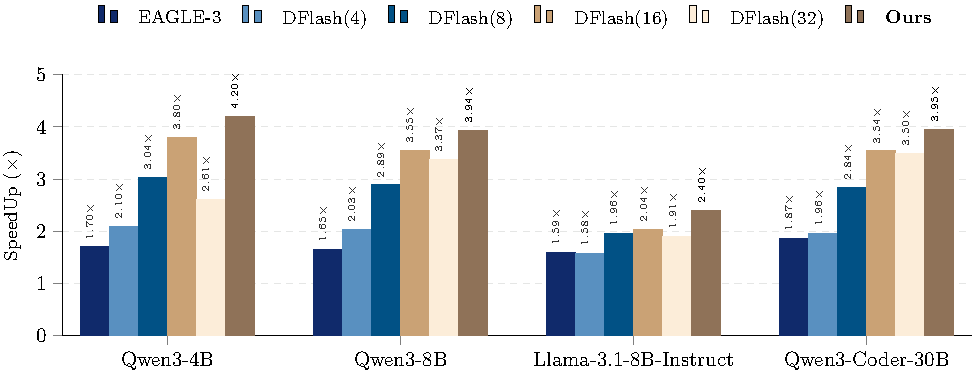
\includegraphics[width=0.95\textwidth]{IMG/comparision4.pdf}
    \caption{Speedup comparison across models under temperature $T=1$. Our method achieves the highest acceleration across all settings. Here, DFlash$(n)$ denotes DFlash with block size $n$.}
    \label{fig:performance_comparision}
\end{figure}



In this paper, we revisit diffusion-based speculative decoding from a largely overlooked perspective. Beyond designing stronger draft models or more efficient verification mechanisms, we ask whether the decoding strategy itself should be treated as a learnable component. We argue that block size is not merely an engineering parameter, but a key control variable that determines the acceptance length in speculative decoding. To validate this insight, we conduct a systematic block size sweep across multiple representative datasets. The results show a clear mismatch between sample-wise optimal block sizes and the fixed configuration used during training. Only a subset of samples achieve optimal performance under the default setting, while many prefer different inference-time block sizes. This suggests that existing fixed strategies fail to fully exploit the efficiency potential of diffusion-based speculative decoding.

Furthermore, we observe that although the optimal block size varies across samples, its distribution is not arbitrarily scattered. Instead, it exhibits a clear local structure: for most samples, the optimal block size concentrates within a narrow region around the training configuration, and few samples achieve optimal performance outside this region. This locality has an important methodological implication. It transforms what would otherwise require expensive online search into a small-scale, discrete, and well-structured classification problem. In other words, sample-adaptive block size selection does not require complex dynamic optimization, and can instead be efficiently handled by a lightweight predictor.

Based on this insight, we introduce BlockPilot, a sample-adaptive block size selection method. Specifically, after the target model completes prefilling, we use the predictive distribution of the final token as a representation of the current decoding state. Since this token has aggregated full-context information via autoregressive attention, its distribution reflects not only local uncertainty but also the model’s estimation of future generation stability, serving as an effective signal for predicting the acceptable block length. Therefore, we formulate block size selection as a policy learning problem over a discrete local action space and approximate the optimal policy with a lightweight predictor. The prediction is performed only once after prefilling and does not modify the target model, draft model, or verification process, allowing seamless integration into existing diffusion-based speculative decoding frameworks. Extensive experiments across models and datasets demonstrate that our method further improves the efficiency of speculative decoding without altering the original inference framework, achieving an acceptance length of 5.92 and a 4.20$\times$ speedup on Qwen3-4B at a temperature of 1. Fig. \ref{fig:performance_comparision} presents the speedup comparison across different methods. Our contributions can be summarized as follows:
\begin{itemize}[leftmargin=*]
    \item We identify decoding policy as a learnable component in diffusion-based speculative decoding, showing that fixed block-size strategies are suboptimal across diverse inputs.
    \item We show that the optimal block size follows a structured local distribution, enabling efficient policy learning over a discrete action space.
    \item We propose BlockPilot, a lightweight instance-adaptive policy learning framework that predicts block size from the prefilling state, achieving consistent speedup gains with minimal overhead.
\end{itemize}







\section{Methodology}
\subsection{Problem Formulation}
Speculative decoding based on diffusion language models \cite{li2025diffuspecunlockingdiffusionlanguage,sandler2025specdiff2scalingdiffusiondrafter,samragh2025llmknowsfutureuncovering,chen2026dflash} is an efficient framework for accelerating autoregressive inference. It trains a lightweight diffusion language model as the draft model with a block size of $B$, and leverages a block-level diffusion mechanism to generate $B$ tokens in parallel. The target autoregressive model then verifies the generated sequence in parallel, alleviating the sequential bottleneck of autoregressive decoding. Formally, within a single speculative decoding step, the average per-token generation latency is defined as follows \cite{chen2026dflash}:
\begin{equation}
L(B) = \frac{T_{\text{draft}}(B) + T_{\text{verify}}(B)}{\tau(B)}
\end{equation}
where $L(B)$ denotes the average token generation latency under block size $B$, $T_{\text{draft}}(B)$ and $T_{\text{verify}}(B)$ represent the computational costs of the draft generation and verification stages, respectively, and $\tau(B)$ denotes the expected number of accepted tokens per verification step. Furthermore, the end-to-end speedup $\eta(B)$ is defined as:
\begin{equation}
\eta(B) = \frac{L_{\text{AR}}}{L(B)}
\end{equation}
where $L_{\text{AR}}$ denotes the average latency of standard autoregressive decoding. Since both draft generation and verification can be executed in a block-parallel manner, $T_{\text{draft}}(B)$ and $T_{\text{verify}}(B)$ typically increase sublinearly with $B$ and can often be approximated as near-constant overhead in practice \cite{hooper2025speed,stern2018blockwise,santilli2023accelerating}. This implies that $\tau(B)$ primarily governs efficiency, suggesting that an optimal inference block size $B^*$ maximizes $\tau(B)$ and improves end-to-end acceleration.

In common settings, inference typically uses the same block size $B$ as in training to maintain consistency between training and inference. However, this choice may be suboptimal at inference time, since the optimal block size can vary across input samples and deviate from the training configuration. To address this issue, we aim to adaptively determine a sample-specific optimal inference block size $B^*$ for each sample, instead of using a fixed training-time block size $B$. Specifically, $B^*$ is defined for each sample as the value that maximizes the expected acceptance length during speculative decoding, thereby improving inference efficiency.

% \begin{figure}[t]
%     \centering
%     \includegraphics[width=0.48\textwidth]{IMG/1.pdf}
% \caption{
% Proportion of samples whose optimal block size $B^*$ matches ($B^* = B$) or mismatches ($B^* \ne B$) the fixed training block size $B$ across multiple datasets.
% }
%     \label{fig:block_size_mismatch}
% \end{figure}
\subsection{Key Findings}
To systematically analyze the impact of block size on speculative decoding performance, we perform an exhaustive sweep over candidate block sizes on multiple representative datasets. This allows us to directly compare decoding behavior under different levels of block-level parallelism. Specifically, we define the candidate set as $\mathcal{B} = \{1, 2, \ldots, 2B\}$, where $B$ denotes the block size used during training. For each input sample $x$, we define its optimal block size as follows:
\begin{equation}
\label{B*}
B^*(x) = \arg\max_{b \in \mathcal{B}} \tau(b; x)
\end{equation}
where $\tau(b; x)$ denotes the average number of accepted tokens for sample $x$ under block size $b$. The acceptance length determines the effective number of generated tokens per decoding step and therefore directly reflects how efficiently the draft tokens are utilized. It thus serves as a key metric for speculative decoding efficiency.

\paragraph{Finding I: Instance-wise Variability of Optimal Block Size.}
We first observe that the sample-wise optimal block size $B^*(x)$ varies significantly across samples, and does not necessarily match the fixed block size $B$ used during training. As shown in Fig.~\ref{fig:block_size_mismatch}, we report the proportions of samples satisfying $B^*(x)=B$ and $B^*(x)\neq B$ for each dataset. The results indicate that only a subset of samples align with the training configuration, while a substantial fraction prefer different block sizes at inference time, and this pattern is consistent across datasets.

These observations suggest that a fixed block size is insufficient to capture optimal decoding behavior across diverse inputs. The variation arises from differences in context structure and predictability: for some inputs, strong structural constraints from the prefilling stage enable high consistency over larger blocks, whereas for others, errors accumulate more rapidly as block size increases, resulting in shorter accepted lengths. This mismatch between the fixed training-time block size and sample-specific optimal decoding behavior motivates sample-adaptive block size selection at inference time.


% \begin{figure}[t]
%     \centering
%     % --- First Subfigure ---
%     \begin{subfigure}[b]{0.48\textwidth}
%         \centering
%         \includegraphics[width=\textwidth]{IMG/2.pdf}
%         \caption{Unimodal distribution of the optimal block size, peaking at the trained block size $B$.}
%         \label{fig:left_plot}
%     \end{subfigure}
%     \hfill
%     % --- Second Subfigure ---
%     \begin{subfigure}[b]{0.48\textwidth}
%         \centering
%         \includegraphics[width=\textwidth]{IMG/3.pdf}
%         \caption{Symmetric bimodal distribution of the optimal block size, with peaks near the trained block size $B$.}
%         \label{fig:right_plot}
%     \end{subfigure}
%     \caption{Distribution patterns of the optimal block size. Both patterns demonstrate strong locality. The discrete block sizes from $B-3$ to $B+3$ cover the optimal block size for nearly all samples.}
%     \label{fig:overall_label}
% \end{figure}


\begin{figure*}[t]
    \centering
    % --- 子图 (a) ---
    \begin{subfigure}[b]{0.32\textwidth}
        \centering
        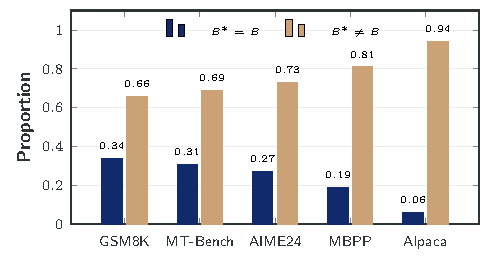
\includegraphics[width=\textwidth]{IMG/1_2_2.pdf}
        \caption{Proportion of samples with $B^*$ matching or mismatching $B$.}
        \label{fig:block_size_mismatch}
    \end{subfigure}
    \hfill
    % --- 子图 (b) ---
    \begin{subfigure}[b]{0.32\textwidth}
        \centering
        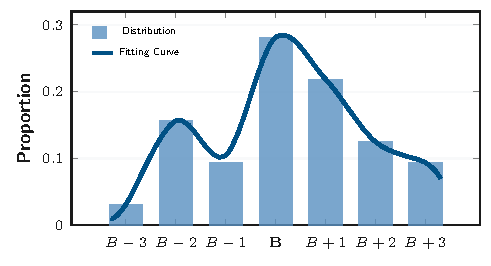
\includegraphics[width=\textwidth]{IMG/22_2.pdf}
        \caption{Unimodal distribution of $B^*$ peaking at the trained size $B$.}
        \label{fig:left_plot}
    \end{subfigure}
    \hfill
    % --- 子图 (c) ---
    \begin{subfigure}[b]{0.32\textwidth}
        \centering
        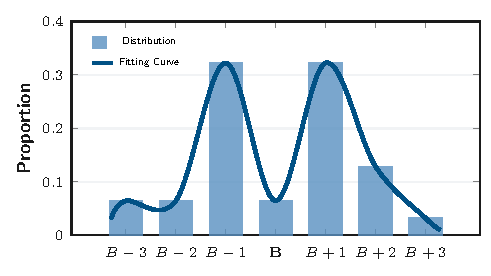
\includegraphics[width=\textwidth]{IMG/22_3.pdf}
        \caption{Symmetric bimodal distribution of $B^*$ near the trained size $B$.}
        \label{fig:right_plot}
    \end{subfigure}

    \caption{Analysis of optimal block size $B^*$. (a) Matching and mismatching proportions across datasets. (b-c) Distribution patterns demonstrating strong locality, where the range $[B-3, B+3]$ covers the optimal size for nearly all samples.}
    \label{fig:overall_label}
\end{figure*}


\paragraph{Finding II: Local Interval Property of Optimal Block Size.}
Although the optimal block size varies across samples, its distribution exhibits a clear local interval structure. As shown in Fig.~\ref{fig:overall_label}, we observe two dominant patterns in the distribution, both indicating strong locality. Fig.~\ref{fig:left_plot} shows a unimodal distribution peaked at the training block size $B$, with probabilities rapidly decaying on both sides. Fig.~\ref{fig:right_plot} instead presents a bimodal but still localized pattern, with both peaks near $B$. Concretely, for almost all samples, the optimal block size satisfies as follows:
\begin{equation}
B^*(x) \in \{B-k, \ldots, B+k\}
\end{equation}
and it covers nearly all cases when $k=3$. Once the block size deviates from $B$ beyond this small range, the acceptance length drops sharply, making such choices rarely optimal. This indicates that the optimal block size exhibits strong locality across samples, with optimal solutions concentrated within a narrow region around the training block size.

This locality has important methodological implications. It reduces the unbounded search space over block sizes to a small discrete interval, within which the optimum almost always lies, significantly simplifying the problem. More importantly, it enables learning-based strategies that select block sizes from a limited candidate set rather than performing global search.


\paragraph{Finding III: Classification Formulation of Block Size Selection.}
% Building on Finding II, which reveals a pronounced local interval structure of the optimal block size around the training block size, we can naturally formulate the sample-adaptive block size selection problem as a structured classification task over a finite discrete space. Specifically, we restrict the candidate set to a local neighborhood $\{B - k, \ldots, B + k\}$, and learn a mapping function that predicts the optimal block size category conditioned on the current input sample. We use the predictive probability distribution of the last token after the prefilling stage as the input representation. This design is motivated by the causal structure of autoregressive decoding: the final token attends to the full context and thus provides a globally aggregated summary of the input sequence. Its predictive distribution captures not only local contextual constraints but also implicit signals of semantic consistency and uncertainty in future generation, making it a strong indicator for block-size selection. Under this formulation, the probability distribution serves as an approximate sufficient statistic with respect to the decision of optimal block size. This allows the classifier to make the decision with a single forward pass. Moreover, the proposed module can be seamlessly integrated into existing speculative decoding frameworks, enabling sample-level adaptive optimization without modifying the generation pipeline.

Building on Finding II, which reveals a strong local interval structure of the optimal block size around the training block size, we formulate sample-adaptive block size selection as a structured classification task over a finite discrete space. Specifically, we restrict the candidate set to a local neighborhood $\{B-k, \ldots, B+k\}$ and learn a mapping function that predicts the optimal block size conditioned on the input sample. We use the predictive probability distribution of the last token after the prefilling stage as the input representation. Motivated by the causal structure of autoregressive decoding, the final token attends to the full context and thus provides a globally aggregated summary of the input sequence. Its predictive distribution captures contextual constraints, semantic consistency, and uncertainty in future generation, making it informative for block-size selection. We also explored using only the Top-$k$ probabilities as input, but this led to severe overfitting \cite{hinton2015distilling,berrada2018smooth}: the training accuracy reached around $80\%$, while the test accuracy remained only about $10\%$. Therefore, we retain the full predictive distribution to preserve richer information and improve generalization. Under this formulation, the probability distribution serves as an approximate sufficient statistic for optimal block size selection, enabling the classifier to make decisions with a single forward pass. Moreover, the proposed module can be seamlessly integrated into existing speculative decoding frameworks without modifying the generation pipeline.

\subsection{Training}
Following the classification formulation of the block size selection problem, the training objective is to learn a mapping function as follows:
\begin{equation}
f : p(x) \rightarrow B^*(x)
\end{equation}
where $p(x)$ denotes the predictive probability distribution of the last token after the prefilling stage for input $x$, and $B^*(x)$ denotes the corresponding optimal block size category. The training process consists of two components: supervised data construction and learning the block size predictor.


\paragraph{Supervised Data Construction.}
Since the optimal block size is not explicitly annotated, we construct supervised data via an offline enumeration strategy. For each input sample $x$, we first run the target model’s prefilling stage and extract the predictive distribution at the last position $p(x)$ as the input feature. Then, over the local candidate set $\mathcal{B} = \{B - k, \ldots, B + k\}$ determined by Finding II, we enumerate each candidate block size $b$ and execute full speculative decoding to measure the corresponding acceptance length $\tau(b; x)$. The block size that yields the maximum acceptance length is taken as the supervision signal, i.e., the optimal block size $B^*(x)$ defined in Eq.~\ref{B*}. Based on this procedure, we construct the training dataset $\mathcal{D}$ as follows:
\begin{equation}
\mathcal{D} = \{(p(x_i), B^*(x_i))\}_{i=1}^N
\end{equation}
In practice, the candidate set is small (typically $2k + 1 $), ensuring that the enumeration cost remains tractable. Since evaluations across different candidate block sizes are mutually independent, the process is highly parallelizable. This data construction procedure directly aligns with the optimization objective of speculative decoding, enabling the model to learn a mapping from decoding states to optimal decisions without relying on hand-crafted heuristics.


\paragraph{Block Size Predictor.}
We adopt a lightweight $n$-layer multilayer perceptron as a lightweight policy network. Since the input feature $p(x)$ is a high-level state representation compressed from the prefilling stage of the target model, sequence modeling architectures are unnecessary. Instead, we employ a simple discriminative model that is computationally efficient and easy to deploy. The model takes $p(x)$ as input and outputs logits over the candidate block size set $\mathcal{B}$. As $p(x)$ already encodes rich contextual information from the target model, a shallow architecture is sufficient to achieve strong performance while introducing only limited latency. The output distribution is defined via a softmax over candidate block sizes:
\begin{equation}
P(b \mid x) = \frac{\exp(o_b)}{\sum_{b' \in \mathcal{B}} \exp(o_{b'})}
\end{equation}
where $o_b$ denotes the logit corresponding to the candidate block size $b \in \mathcal{B}$. The model is trained by minimizing the standard cross-entropy loss over the training dataset:
\begin{equation}
L = -\frac{1}{N} \sum_{i=1}^{N} \log P\!\left(B^*(x_i)\mid x_i\right)
\end{equation}
where $N$ denotes the number of training samples and $B^*(x_i)$ represents the ground-truth optimal block size for sample $x_i$. This objective encourages the model to assign higher probability mass to the optimal block size, thereby learning a direct mapping from decoding states to optimal decisions. Owing to the compact design of the predictor, both training and inference incur relatively low computational overhead.





\begin{figure}[t]
    \centering
    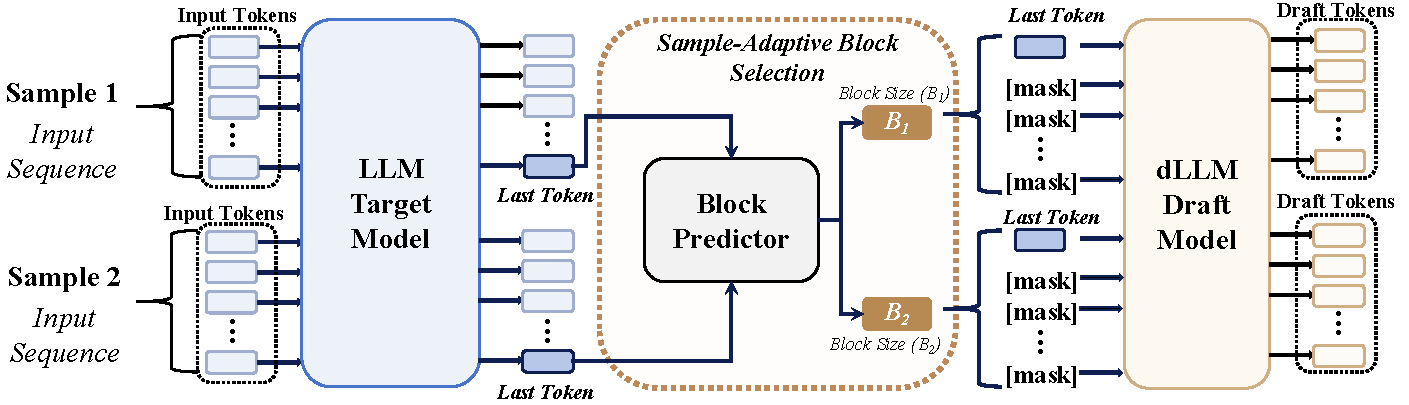
\includegraphics[width=1\textwidth]{IMG/Overview3.pdf}
    \caption{Overview of the BlockPilot inference pipeline. Given an input sequence, the target LLM performs prefilling and produces the predictive distribution of the last token, which serves as a compact representation of the decoding state. This distribution is then fed into a lightweight block size predictor to determine an instance-specific block size. Based on the predicted block size, the diffusion-based draft model generates a block of draft tokens in parallel.}
    \label{fig:inference}
\end{figure}

\subsection{Inference}



\begin{wraptable}{r}{0.46\textwidth}
\vspace{-8pt}
\centering
\small
\setlength{\tabcolsep}{3.2pt} 
\renewcommand{\arraystretch}{1.15} 
\caption{Overhead analysis of the block size predictor compared to backbone models.}
\label{tab:model_efficiency}
\resizebox{0.46\textwidth}{!}{%
\begin{tabular}{l c rr r}
\toprule
\multirow{2}{*}{\textbf{Model}} & \multirow{2}{*}{\textbf{\#Params}} & \multicolumn{2}{c}{\textbf{Memory}} & \multirow{2}{*}{\textbf{Latency}} \\
\cmidrule(l{2pt}r{2pt}){3-4} 
& & \textbf{Act.} & \textbf{Param.} & \\
\midrule
Qwen3-4B              & 4.41B & 6.53 GB & 8.62 GB  & 183.48 ms \\
\rowcolor{gray!10}
Qwen3-8B              & 8.19B & 8.16 GB & 16.00 GB & 278.37 ms \\
Llama-3.1-8B-Instruct & 8.03B & 7.10 GB & 15.68 GB & 272.14 ms \\
\midrule
\rowcolor[HTML]{ecf2f9}
\textit{Block Size Predictor} & 0.32B & 0.02 MB & 0.62 GB & 7.34 ms \\
\bottomrule
\end{tabular}%
}
\vspace{-8pt}
\end{wraptable}
During inference, we integrate the learned block size predictor into the speculative decoding pipeline to enable sample-wise adaptive block size selection. Given an input sample $x$, we run the prefilling stage of the target model and extract the predictive distribution at the last position, denoted as $p(x)$. The predictor then produces logits over the candidate set $\mathcal{B}$, and the block size is determined as follows:
\begin{equation}
\hat{B}(x) = \arg\max_{b \in \mathcal{B}} f(p(x))_b
\end{equation}
where $f(p(x))_b$ denotes the predicted score for candidate block size $b$. Once $\hat{B}(x)$ is obtained, it is fixed for the entire subsequent speculative decoding process, including both draft generation and target model verification. Fig. \ref{fig:inference} presents an overview of the inference process. Compared to fixed block size strategies, this approach adaptively selects a more suitable level of parallel generation conditioned on each input sample. Notably, the block size prediction is performed only once after the prefilling stage, and the predictor itself is implemented as a lightweight network, resulting in minimal computational overhead. Table~\ref{tab:model_efficiency} compares the predictor with the backbone model in terms of parameter size, memory footprint, and inference latency, showing that the predictor introduces only millisecond-level latency. Although the predictor introduces a small additional memory footprint, this cost is minor compared with the backbone models and is well compensated by the resulting speedup. Therefore, the small additional memory overhead represents a favorable trade-off for improving decoding efficiency.






% \begin{table*}[t]
% \centering
% \scriptsize
% \setlength{\tabcolsep}{3.0pt}
% \renewcommand{\arraystretch}{1.14}
% \caption{Speedup ratios and average acceptance length $\tau$ on Qwen3 models across Math, Code, and Chat benchmarks. Q3-4B and Q3-8B denote Qwen3-4B and Qwen3-8B, respectively. DFlash$(n)$ denotes DFlash with block size $n$.}
% \label{tab:qwen3_speedup_acceptance}
% \resizebox{\textwidth}{!}{%
% \begin{tabular}{@{}ll*{8}{cc}@{}}
% \toprule
% \multirow{2}{*}{\textbf{Model}}
% & \multirow{2}{*}{\textbf{Method}}
% & \multicolumn{6}{c}{\textbf{Math}}
% & \multicolumn{6}{c}{\textbf{Code}}
% & \multicolumn{2}{c}{\textbf{Chat}}
% & \multicolumn{2}{c}{\textbf{Overall}} \\
% \cmidrule(lr){3-8}
% \cmidrule(lr){9-14}
% \cmidrule(lr){15-16}
% \cmidrule(l){17-18}
% &
% & \multicolumn{2}{c}{GSM8K}
% & \multicolumn{2}{c}{MATH-500}
% & \multicolumn{2}{c}{AIME24}
% & \multicolumn{2}{c}{HumanEval}
% & \multicolumn{2}{c}{MBPP}
% & \multicolumn{2}{c}{SWE-Bench}
% & \multicolumn{2}{c}{MT-Bench}
% & \multicolumn{2}{c}{Avg.} \\
% \midrule
% \multicolumn{2}{@{}l}{\textit{Temperature} $=0$}
% & \textit{Speedup} & $\tau$
% & \textit{Speedup} & $\tau$
% & \textit{Speedup} & $\tau$
% & \textit{Speedup} & $\tau$
% & \textit{Speedup} & $\tau$
% & \textit{Speedup} & $\tau$
% & \textit{Speedup} & $\tau$
% & \textit{Speedup} & $\tau$ \\
% \midrule
% \multirow{6}{*}{Q3-4B}
% & EAGLE-3     & 1.99$\times$ & 3.30 & 1.83$\times$ & 3.08 & 1.79$\times$ & 3.05 & 1.84$\times$ & 3.05 & 1.78$\times$ & 2.95 & 1.39$\times$ & 2.48 & 1.74$\times$ & 3.02 & 1.70$\times$ & 2.95 \\
% & DFlash (4)  & 2.29$\times$ & 3.32 & 2.20$\times$ & 3.48 & 2.12$\times$ & 3.45 & 2.12$\times$ & 3.22 & 2.16$\times$ & 3.17 & 1.59$\times$ & 2.58 & 1.45$\times$ & 2.85 & 1.99$\times$ & 3.15 \\
% & DFlash (8)  & 3.56$\times$ & 5.16 & 3.59$\times$ & 5.68 & 3.47$\times$ & 5.64 & 3.19$\times$ & 4.84 & 3.22$\times$ & 4.71 & 1.95$\times$ & 3.17 & 1.99$\times$ & 3.91 & 2.99$\times$ & 4.73 \\
% & DFlash (16) & 4.55$\times$ & 6.59 & 5.25$\times$ & 8.31 & 4.58$\times$ & 7.45 & 4.28$\times$ & 6.51 & 4.26$\times$ & 6.24 & 2.33$\times$ & 3.78 & 2.69$\times$ & 5.29 & 3.99$\times$ & 6.31 \\
% & DFlash (32) & 2.92$\times$ & 4.24 & 3.22$\times$ & 5.09 & 2.99$\times$ & 4.86 & 2.56$\times$ & 3.89 & 2.71$\times$ & 3.97 & 1.69$\times$ & 2.74 & 1.62$\times$ & 3.19 & 2.53$\times$ & 4.00 \\
% & \textbf{Ours} & \textbf{4.76$\times$} & \textbf{6.90} & \textbf{5.45$\times$} & \textbf{8.62} & \textbf{4.80$\times$} & \textbf{7.82} & \textbf{4.46$\times$} & \textbf{6.77} & \textbf{4.38$\times$} & \textbf{6.42} & \textbf{2.45$\times$} & \textbf{3.98} & \textbf{2.85$\times$} & \textbf{5.62} & \textbf{4.17$\times$} & \textbf{6.59} \\
% \midrule
% \multirow{6}{*}{Q3-8B}
% & EAGLE-3     & 1.94$\times$ & 3.23 & 1.81$\times$ & 3.02 & 1.79$\times$ & 3.00 & 1.89$\times$ & 3.17 & 1.69$\times$ & 2.82 & 1.47$\times$ & 2.45 & 1.63$\times$ & 2.83 & 1.75$\times$ & 2.93 \\
% & DFlash (4)  & 2.45$\times$ & 3.29 & 2.50$\times$ & 3.47 & 2.55$\times$ & 3.44 & 2.45$\times$ & 3.33 & 2.32$\times$ & 3.21 & 1.96$\times$ & 2.58 & 1.51$\times$ & 2.58 & 2.25$\times$ & 3.13 \\
% & DFlash (8)  & 3.76$\times$ & 5.04 & 4.09$\times$ & 5.67 & 4.22$\times$ & 5.69 & 3.82$\times$ & 5.19 & 3.51$\times$ & 4.86 & 2.45$\times$ & 3.23 & 2.01$\times$ & 3.45 & 3.41$\times$ & 4.73 \\
% & DFlash (16) & 4.89$\times$ & 6.56 & 5.98$\times$ & 8.29 & 5.57$\times$ & 7.51 & 4.98$\times$ & 6.76 & 4.33$\times$ & 5.99 & 2.72$\times$ & 3.58 & 2.48$\times$ & 4.25 & 4.42$\times$ & 6.13 \\
% & DFlash (32) & 4.47$\times$ & 5.99 & 5.66$\times$ & 7.84 & 5.20$\times$ & 7.01 & 4.66$\times$ & 6.32 & 3.92$\times$ & 5.42 & 2.50$\times$ & 3.29 & 2.37$\times$ & 4.06 & 4.11$\times$ & 5.70 \\
% & \textbf{Ours} & \textbf{5.02$\times$} & \textbf{6.73} & \textbf{6.17$\times$} & \textbf{8.56} & \textbf{6.16$\times$} & \textbf{8.30} & \textbf{5.21$\times$} & \textbf{7.07} & \textbf{4.53$\times$} & \textbf{6.26} & \textbf{2.96$\times$} & \textbf{3.90} & \textbf{2.55$\times$} & \textbf{4.37} & \textbf{4.66$\times$} & \textbf{6.46} \\
% \midrule
% \multicolumn{2}{@{}l}{\textit{Temperature} $=1$}
% & \textit{Speedup} & $\tau$
% & \textit{Speedup} & $\tau$
% & \textit{Speedup} & $\tau$
% & \textit{Speedup} & $\tau$
% & \textit{Speedup} & $\tau$
% & \textit{Speedup} & $\tau$
% & \textit{Speedup} & $\tau$
% & \textit{Speedup} & $\tau$ \\
% \midrule
% \multirow{6}{*}{Q3-4B}
% & EAGLE-3     & 1.89$\times$ & 3.22 & 1.75$\times$ & 2.99 & 1.64$\times$ & 2.79 & 1.74$\times$ & 3.01 & 1.69$\times$ & 2.89 & 1.47$\times$ & 2.31 & 1.77$\times$ & 2.99 & 1.70$\times$ & 2.88 \\
% & DFlash (4)  & 2.32$\times$ & 3.17 & 2.34$\times$ & 3.26 & 2.08$\times$ & 2.90 & 2.29$\times$ & 3.11 & 2.25$\times$ & 3.10 & 1.79$\times$ & 2.36 & 1.62$\times$ & 2.74 & 2.10$\times$ & 2.95 \\
% & DFlash (8)  & 3.60$\times$ & 4.91 & 3.71$\times$ & 5.16 & 2.97$\times$ & 4.13 & 3.37$\times$ & 4.58 & 3.21$\times$ & 4.42 & 2.17$\times$ & 2.86 & 2.24$\times$ & 3.79 & 3.04$\times$ & 4.26 \\
% & DFlash (16) & 4.36$\times$ & 5.95 & 4.83$\times$ & 6.72 & 3.66$\times$ & 5.10 & 4.32$\times$ & 5.87 & 4.02$\times$ & 5.54 & 2.33$\times$ & 3.07 & 3.10$\times$ & 5.23 & 3.80$\times$ & 5.35 \\
% & DFlash (32) & 2.83$\times$ & 3.87 & 3.35$\times$ & 4.66 & 2.79$\times$ & 3.88 & 2.76$\times$ & 3.76 & 2.69$\times$ & 3.71 & 1.91$\times$ & 2.52 & 1.91$\times$ & 3.22 & 2.61$\times$ & 3.66 \\
% & \textbf{Ours} & \textbf{4.77$\times$} & \textbf{6.51} & \textbf{5.41$\times$} & \textbf{7.53} & \textbf{4.02$\times$} & \textbf{5.60} & \textbf{4.74$\times$} & \textbf{6.45} & \textbf{4.59$\times$} & \textbf{6.33} & \textbf{2.58$\times$} & \textbf{3.39} & \textbf{3.31$\times$} & \textbf{5.59} & \textbf{4.20$\times$} & \textbf{5.92} \\
% \midrule
% \multirow{6}{*}{Q3-8B}
% & EAGLE-3     & 1.87$\times$ & 3.12 & 1.73$\times$ & 2.91 & 1.63$\times$ & 2.74 & 1.75$\times$ & 3.05 & 1.64$\times$ & 2.74 & 1.33$\times$ & 2.11 & 1.58$\times$ & 2.70 & 1.65$\times$ & 2.77 \\
% & DFlash (4)  & 2.34$\times$ & 3.17 & 2.25$\times$ & 3.22 & 2.05$\times$ & 2.92 & 2.25$\times$ & 3.05 & 2.23$\times$ & 3.03 & 1.66$\times$ & 2.20 & 1.44$\times$ & 2.45 & 2.03$\times$ & 2.86 \\
% & DFlash (8)  & 3.48$\times$ & 4.72 & 3.53$\times$ & 5.06 & 2.92$\times$ & 4.17 & 3.26$\times$ & 4.41 & 3.20$\times$ & 4.36 & 1.94$\times$ & 2.57 & 1.93$\times$ & 3.28 & 2.89$\times$ & 4.08 \\
% & DFlash (16) & 4.28$\times$ & 5.81 & 4.62$\times$ & 6.62 & 3.49$\times$ & 4.98 & 4.19$\times$ & 5.68 & 3.98$\times$ & 5.41 & 2.09$\times$ & 2.77 & 2.20$\times$ & 3.75 & 3.55$\times$ & 5.00 \\
% & DFlash (32) & 4.10$\times$ & 5.57 & 4.41$\times$ & 6.32 & 3.39$\times$ & 4.84 & 3.77$\times$ & 5.11 & 3.68$\times$ & 5.00 & 2.01$\times$ & 2.67 & 2.23$\times$ & 3.79 & 3.37$\times$ & 4.75 \\
% & \textbf{Ours} & \textbf{4.69$\times$} & \textbf{6.37} & \textbf{5.06$\times$} & \textbf{7.25} & \textbf{3.84$\times$} & \textbf{5.47} & \textbf{4.65$\times$} & \textbf{6.30} & \textbf{4.54$\times$} & \textbf{6.17} & \textbf{2.30$\times$} & \textbf{3.05} & \textbf{2.48$\times$} & \textbf{4.23} & \textbf{3.94$\times$} & \textbf{5.55} \\
% \bottomrule
% \end{tabular}%
% }
% \end{table*}

\begin{table*}[t]
\centering
\scriptsize
\setlength{\tabcolsep}{3.0pt}
\renewcommand{\arraystretch}{1.14}
\caption{Speedup ratios and average acceptance length $\tau$ on Qwen3 models across Math, Code, and Chat benchmarks. Q3-4B and Q3-8B denote Qwen3-4B and Qwen3-8B, respectively. DFlash$(n)$ denotes DFlash with block size $n$.}
\label{tab:qwen3_speedup_acceptance}
\resizebox{\textwidth}{!}{%
\begin{tabular}{@{}ll*{8}{cc}@{}}
\toprule
\multirow{2}{*}{\textbf{Model}}
& \multirow{2}{*}{\textbf{Method}}
& \multicolumn{6}{c}{\textbf{Math}}
& \multicolumn{6}{c}{\textbf{Code}}
& \multicolumn{2}{c}{\textbf{Chat}}
& \multicolumn{2}{c}{\textbf{Overall}} \\
\cmidrule(lr){3-8}
\cmidrule(lr){9-14}
\cmidrule(lr){15-16}
\cmidrule(l){17-18}
&
& \multicolumn{2}{c}{GSM8K}
& \multicolumn{2}{c}{MATH-500}
& \multicolumn{2}{c}{AIME24}
& \multicolumn{2}{c}{HumanEval}
& \multicolumn{2}{c}{MBPP}
& \multicolumn{2}{c}{SWE-Bench}
& \multicolumn{2}{c}{MT-Bench}
& \multicolumn{2}{c}{Avg.} \\
\midrule
\multicolumn{2}{@{}l}{\textit{Temperature} $=0$}
& \textit{Speedup} & $\tau$
& \textit{Speedup} & $\tau$
& \textit{Speedup} & $\tau$
& \textit{Speedup} & $\tau$
& \textit{Speedup} & $\tau$
& \textit{Speedup} & $\tau$
& \textit{Speedup} & $\tau$
& \textit{Speedup} & $\tau$ \\
\midrule
\multirow{6}{*}{Q3-4B}
& EAGLE-3     & 1.99$\times$ & 3.30 & 1.83$\times$ & 3.08 & 1.79$\times$ & 3.05 & 1.84$\times$ & 3.05 & 1.78$\times$ & 2.95 & 1.39$\times$ & 2.48 & 1.74$\times$ & 3.02 & 1.70$\times$ & 2.95 \\
& DFlash (4)  & 2.29$\times$ & 3.32 & 2.20$\times$ & 3.48 & 2.12$\times$ & 3.45 & 2.12$\times$ & 3.22 & 2.16$\times$ & 3.17 & 1.59$\times$ & 2.58 & 1.45$\times$ & 2.85 & 1.99$\times$ & 3.15 \\
& DFlash (8)  & 3.56$\times$ & 5.16 & 3.59$\times$ & 5.68 & 3.47$\times$ & 5.64 & 3.19$\times$ & 4.84 & 3.22$\times$ & 4.71 & 1.95$\times$ & 3.17 & 1.99$\times$ & 3.91 & 2.99$\times$ & 4.73 \\
& DFlash (16) & 4.55$\times$ & 6.59 & 5.25$\times$ & 8.31 & 4.58$\times$ & 7.45 & 4.28$\times$ & 6.51 & 4.26$\times$ & 6.24 & 2.33$\times$ & 3.78 & 2.69$\times$ & 5.29 & 3.99$\times$ & 6.31 \\
& DFlash (32) & 2.92$\times$ & 4.24 & 3.22$\times$ & 5.09 & 2.99$\times$ & 4.86 & 2.56$\times$ & 3.89 & 2.71$\times$ & 3.97 & 1.69$\times$ & 2.74 & 1.62$\times$ & 3.19 & 2.53$\times$ & 4.00 \\
& \textbf{BlockPilot} & \textbf{4.76$\times$} & \textbf{6.90} & \textbf{5.45$\times$} & \textbf{8.62} & \textbf{4.80$\times$} & \textbf{7.82} & \textbf{4.46$\times$} & \textbf{6.77} & \textbf{4.38$\times$} & \textbf{6.42} & \textbf{2.45$\times$} & \textbf{3.98} & \textbf{2.85$\times$} & \textbf{5.62} & \textbf{4.17$\times$} & \textbf{6.59} \\
\midrule
\multirow{6}{*}{Q3-8B}
& EAGLE-3     & 1.94$\times$ & 3.23 & 1.81$\times$ & 3.02 & 1.79$\times$ & 3.00 & 1.89$\times$ & 3.17 & 1.69$\times$ & 2.82 & 1.47$\times$ & 2.45 & 1.63$\times$ & 2.83 & 1.75$\times$ & 2.93 \\
& DFlash (4)  & 2.45$\times$ & 3.29 & 2.50$\times$ & 3.47 & 2.55$\times$ & 3.44 & 2.45$\times$ & 3.33 & 2.32$\times$ & 3.21 & 1.96$\times$ & 2.58 & 1.51$\times$ & 2.58 & 2.25$\times$ & 3.13 \\
& DFlash (8)  & 3.76$\times$ & 5.04 & 4.09$\times$ & 5.67 & 4.22$\times$ & 5.69 & 3.82$\times$ & 5.19 & 3.51$\times$ & 4.86 & 2.45$\times$ & 3.23 & 2.01$\times$ & 3.45 & 3.41$\times$ & 4.73 \\
& DFlash (16) & 4.89$\times$ & 6.56 & 5.98$\times$ & 8.29 & 5.57$\times$ & 7.51 & 4.98$\times$ & 6.76 & 4.33$\times$ & 5.99 & 2.72$\times$ & 3.58 & 2.48$\times$ & 4.25 & 4.42$\times$ & 6.13 \\
& DFlash (32) & 4.47$\times$ & 5.99 & 5.66$\times$ & 7.84 & 5.20$\times$ & 7.01 & 4.66$\times$ & 6.32 & 3.92$\times$ & 5.42 & 2.50$\times$ & 3.29 & 2.37$\times$ & 4.06 & 4.11$\times$ & 5.70 \\
& \textbf{BlockPilot} & \textbf{5.02$\times$} & \textbf{6.73} & \textbf{6.17$\times$} & \textbf{8.56} & \textbf{6.16$\times$} & \textbf{8.30} & \textbf{5.21$\times$} & \textbf{7.07} & \textbf{4.53$\times$} & \textbf{6.26} & \textbf{2.96$\times$} & \textbf{3.90} & \textbf{2.55$\times$} & \textbf{4.37} & \textbf{4.66$\times$} & \textbf{6.46} \\
\midrule
\multicolumn{2}{@{}l}{\textit{Temperature} $=1$}
& \textit{Speedup} & $\tau$
& \textit{Speedup} & $\tau$
& \textit{Speedup} & $\tau$
& \textit{Speedup} & $\tau$
& \textit{Speedup} & $\tau$
& \textit{Speedup} & $\tau$
& \textit{Speedup} & $\tau$
& \textit{Speedup} & $\tau$ \\
\midrule
\multirow{6}{*}{Q3-4B}
& EAGLE-3     & 1.89$\times$ & 3.22 & 1.75$\times$ & 2.99 & 1.64$\times$ & 2.79 & 1.74$\times$ & 3.01 & 1.69$\times$ & 2.89 & 1.47$\times$ & 2.31 & 1.77$\times$ & 2.99 & 1.70$\times$ & 2.88 \\
& DFlash (4)  & 2.32$\times$ & 3.17 & 2.34$\times$ & 3.26 & 2.08$\times$ & 2.90 & 2.29$\times$ & 3.11 & 2.25$\times$ & 3.10 & 1.79$\times$ & 2.36 & 1.62$\times$ & 2.74 & 2.10$\times$ & 2.95 \\
& DFlash (8)  & 3.60$\times$ & 4.91 & 3.71$\times$ & 5.16 & 2.97$\times$ & 4.13 & 3.37$\times$ & 4.58 & 3.21$\times$ & 4.42 & 2.17$\times$ & 2.86 & 2.24$\times$ & 3.79 & 3.04$\times$ & 4.26 \\
& DFlash (16) & 4.36$\times$ & 5.95 & 4.83$\times$ & 6.72 & 3.66$\times$ & 5.10 & 4.32$\times$ & 5.87 & 4.02$\times$ & 5.54 & 2.33$\times$ & 3.07 & 3.10$\times$ & 5.23 & 3.80$\times$ & 5.35 \\
& DFlash (32) & 2.83$\times$ & 3.87 & 3.35$\times$ & 4.66 & 2.79$\times$ & 3.88 & 2.76$\times$ & 3.76 & 2.69$\times$ & 3.71 & 1.91$\times$ & 2.52 & 1.91$\times$ & 3.22 & 2.61$\times$ & 3.66 \\
& \textbf{BlockPilot} & \textbf{4.77$\times$} & \textbf{6.51} & \textbf{5.41$\times$} & \textbf{7.53} & \textbf{4.02$\times$} & \textbf{5.60} & \textbf{4.74$\times$} & \textbf{6.45} & \textbf{4.59$\times$} & \textbf{6.33} & \textbf{2.58$\times$} & \textbf{3.39} & \textbf{3.31$\times$} & \textbf{5.59} & \textbf{4.20$\times$} & \textbf{5.92} \\
\midrule
\multirow{6}{*}{Q3-8B}
& EAGLE-3     & 1.87$\times$ & 3.12 & 1.73$\times$ & 2.91 & 1.63$\times$ & 2.74 & 1.75$\times$ & 3.05 & 1.64$\times$ & 2.74 & 1.33$\times$ & 2.11 & 1.58$\times$ & 2.70 & 1.65$\times$ & 2.77 \\
& DFlash (4)  & 2.34$\times$ & 3.17 & 2.25$\times$ & 3.22 & 2.05$\times$ & 2.92 & 2.25$\times$ & 3.05 & 2.23$\times$ & 3.03 & 1.66$\times$ & 2.20 & 1.44$\times$ & 2.45 & 2.03$\times$ & 2.86 \\
& DFlash (8)  & 3.48$\times$ & 4.72 & 3.53$\times$ & 5.06 & 2.92$\times$ & 4.17 & 3.26$\times$ & 4.41 & 3.20$\times$ & 4.36 & 1.94$\times$ & 2.57 & 1.93$\times$ & 3.28 & 2.89$\times$ & 4.08 \\
& DFlash (16) & 4.28$\times$ & 5.81 & 4.62$\times$ & 6.62 & 3.49$\times$ & 4.98 & 4.19$\times$ & 5.68 & 3.98$\times$ & 5.41 & 2.09$\times$ & 2.77 & 2.20$\times$ & 3.75 & 3.55$\times$ & 5.00 \\
& DFlash (32) & 4.10$\times$ & 5.57 & 4.41$\times$ & 6.32 & 3.39$\times$ & 4.84 & 3.77$\times$ & 5.11 & 3.68$\times$ & 5.00 & 2.01$\times$ & 2.67 & 2.23$\times$ & 3.79 & 3.37$\times$ & 4.75 \\
& \textbf{BlockPilot} & \textbf{4.69$\times$} & \textbf{6.37} & \textbf{5.06$\times$} & \textbf{7.25} & \textbf{3.84$\times$} & \textbf{5.47} & \textbf{4.65$\times$} & \textbf{6.30} & \textbf{4.54$\times$} & \textbf{6.17} & \textbf{2.30$\times$} & \textbf{3.05} & \textbf{2.48$\times$} & \textbf{4.23} & \textbf{3.94$\times$} & \textbf{5.55} \\
\bottomrule
\end{tabular}%
}
\end{table*}

\section{Experiments}
\label{Experiments}
\subsection{Experimental Setup}
\paragraph{Models and Benchmarks.}
We evaluate our method on four representative LLMs: Qwen3-4B, Qwen3-8B \cite{yang2025qwen3}, Llama-3.1-8B-Instruct \cite{grattafiori2024llama}, and Qwen3-Coder-30B-A3B \cite{cao2026qwen3}, spanning diverse scales and domains, including both general-purpose instruction-tuned and code-specialized models. We consider benchmarks across three task categories. For mathematical reasoning, we use GSM8K~\citep{cobbe2021training}, MATH-500~\citep{lightman2023let}, and AIME24~\citep{AIME}. For code generation and software engineering, we adopt HumanEval~\citep{chen2021evaluating}, MBPP~\citep{austin2021program}, and SWE-Bench~\citep{jimenez2023swe}. For conversational generation, we use MT-Bench~\citep{zheng2023judging}. Together, these benchmarks cover Math, Code, and Chat scenarios.

\paragraph{Baselines.}
We compare our method with standard autoregressive decoding (baseline), the most classical speculative decoding method with an autoregressive drafter, EAGLE-3~\citep{li2025eagle3scalinginferenceacceleration}, and the state-of-the-art (SOTA) diffusion-based counterpart, DFlash~\citep{chen2026dflash}. Here, DFlash$(n)$ denotes DFlash with block size $n$.

\paragraph{Metrics.}
Since our method preserves the exact output distribution of the target model under speculative decoding, generation quality remains unchanged. Therefore, we focus on efficiency metrics, measured using the following metrics:
\begin{itemize}[leftmargin=*]
    \item \textbf{Average Acceptance Length $\tau$:} The average number of tokens accepted from the draft model per drafting-verification cycle.
    \item \textbf{Speedup Ratio:} The ratio of inference time for standard autoregressive decoding to that for different speculative decoding methods.
\end{itemize}


\paragraph{Implementation Details.}
Our experiments are conducted using the PyTorch framework \citep{paszke2019pytorch} and the Hugging Face Transformers library \citep{wolf2020transformers}, running on NVIDIA H100 80GB GPUs. We construct the training dataset from ShareGPT \cite{chen2024sharegpt4v}, WSC \cite{levesque2012winograd}, and COPA \cite{roemmele2011choice}. We train the model for 100 epochs using the Adam optimizer with a learning rate of $1e^{-5}$. The predictor network consists of two layers with a hidden dimension of 2048, and the default value of the hyperparameter $k$ is set to 2.


\subsection{Main Results}
% Table~\ref{tab:qwen3_speedup_acceptance} presents the main results on the Qwen3 series models under both deterministic decoding and stochastic sampling settings. Overall, our method consistently achieves the best performance across models, temperatures, and benchmark categories. On Qwen3-4B, it reaches average speedups of 4.17$\times$ and 4.20$\times$ under temperature $=0$ and temperature $=1$, respectively. On Qwen3-8B, it achieves 4.66$\times$ and 3.94$\times$ under the two settings. These results outperform EAGLE-3 and all fixed-block DFlash variants, demonstrating the effectiveness of sample-adaptive block size selection.

% Compared with the strongest fixed-block DFlash baseline, our method further improves both speedup and average acceptance length $\tau$. Under temperature $=0$, DFlash(16) is generally the best fixed-block baseline. On Qwen3-4B, our method improves the average speedup from 3.99$\times$ to 4.17$\times$ and increases $\tau$ from 6.31 to 6.59. On Qwen3-8B, the speedup increases from 4.42$\times$ to 4.66$\times$, while $\tau$ improves from 6.13 to 6.46. Similar gains are observed under temperature $=1$, where our method improves the average speedup from 3.80$\times$ to 4.20$\times$ on Qwen3-4B and from 3.55$\times$ to 3.94$\times$ on Qwen3-8B. These results highlight the limitation of fixed-block inference. Although larger block sizes provide more parallelism, they do not always lead to better acceleration. For example, DFlash(32) often underperforms DFlash(16), suggesting that overly large blocks may reduce acceptance length due to accumulated drafting errors. In contrast, our method selects a more suitable block size for each input sample, improving the balance between drafting parallelism and verification acceptance.

% Across Math, Code, and Chat benchmarks, our method remains consistently effective. The gains are also preserved under temperature $=1$, where generation is more stochastic and draft-token acceptance becomes more challenging. This suggests that the last-token predictive distribution after prefilling provides a useful signal for adaptive block size selection. More results are provided in Appendix~\ref{app:main}.


Table~\ref{tab:qwen3_speedup_acceptance} presents the main results on the Qwen3 series models under both deterministic decoding and stochastic sampling settings. Notably, these improvements are achieved without modifying either the draft or target models and introduce only negligible additional latency.  Overall, BlockPilot consistently achieves the best performance across models, temperatures, and benchmark categories. On Qwen3-4B, it reaches average speedups of 4.17$\times$ and 4.20$\times$ under temperature $=0$ and temperature $=1$, respectively. On Qwen3-8B, it achieves 4.66$\times$ and 3.94$\times$ under the two settings. These results outperform EAGLE-3 and all fixed-block DFlash variants, demonstrating the effectiveness of sample-adaptive block size selection. This indicates that the proposed adaptive strategy generalizes well across different model scales and decoding regimes.

Compared with the strongest fixed-block DFlash baseline, BlockPilot further improves both speedup and average acceptance length $\tau$. Under temperature $=0$, DFlash(16) is generally the best fixed-block baseline. On Qwen3-4B, our method improves the average speedup from 3.99$\times$ to 4.17$\times$ and increases $\tau$ from 6.31 to 6.59. On Qwen3-8B, the speedup rises from 4.42$\times$ to 4.66$\times$, while $\tau$ improves from 6.13 to 6.46. Similar gains are observed under temperature $=1$, where our method improves the average speedup from 3.80$\times$ to 4.20$\times$ on Qwen3-4B and from 3.55$\times$ to 3.94$\times$ on Qwen3-8B. These results reveal the limitation of fixed-block inference: larger blocks provide more parallelism, but do not always yield better acceleration. For example, DFlash(32) often underperforms DFlash(16), suggesting that overly large blocks may reduce acceptance due to accumulated drafting errors. In contrast, our method selects a suitable block size for each input sample, better balancing drafting parallelism and verification acceptance.

Across Math, Code, and Chat benchmarks, our method remains consistently effective. The gains are also preserved under temperature $=1$, where generation is more stochastic and draft-token acceptance becomes more challenging. This suggests that the last-token predictive distribution after prefilling provides a useful signal for adaptive block size selection. More results are provided in Appendix~\ref{app:main}.

% Table~\ref{tab:qwen3_speedup_acceptance} reports the main results on the Qwen3 series models. Our method achieves the highest average speedup on both Qwen3-4B and Qwen3-8B. Under temperature $=0$, it reaches average speedups of 4.17$\times$ and 4.66$\times$, respectively. Under temperature $=1$, it achieves 4.20$\times$ and 3.94$\times$, consistently outperforming EAGLE-3 and all DFlash variants with fixed block sizes. Compared with fixed-block DFlash baselines, our method improves both speedup and average acceptance length $\tau$ on most benchmarks. For example, under temperature $=0$, the average acceptance length on Qwen3-4B increases from 6.31 with DFlash(16) to 6.59 with our method, and on Qwen3-8B, it improves from 6.13 to 6.46.

% These results indicate that fixed block size cannot always match sample-wise optimal acceptance behavior, while adaptive block size selection can more effectively improve draft token acceptance. Across task categories, our method consistently performs best on Math, Code, and Chat benchmarks. The gains hold under both decoding settings, showing that the proposed strategy is effective across different task distributions. Moreover, under temperature $=1$ sampling setting, our method remains ahead of all baselines, suggesting that adaptive block size selection remains effective under higher generation uncertainty. More results are provided in Appendix~\ref{app:main}.






\subsection{Ablation Studies}
We conduct ablation studies on Qwen3-4B under a zero-temperature setting to analyze the key design choices of our method, including the predictor architecture, input preprocessing, and candidate interval radius, in order to better understand their impact on performance.




\paragraph{Predictor Configuration.}

\begin{wraptable}{r}{0.46\textwidth}
\vspace{-8pt}
\centering
\scriptsize
\setlength{\tabcolsep}{3.2pt}
\renewcommand{\arraystretch}{1.03}
\caption{Speedup and acceptance length ($\tau$) under different predictor configurations.}
\label{tab:predictor_config}
\resizebox{0.46\textwidth}{!}{%
\begin{tabular}{lcccccc}
\toprule
\multirow{2}{*}{Setting}
& \multicolumn{2}{c}{GSM8K}
& \multicolumn{2}{c}{HumanEval}
& \multicolumn{2}{c}{MT-Bench} \\
\cmidrule(lr){2-3}\cmidrule(lr){4-5}\cmidrule(lr){6-7}
& \textit{Speedup} & $\tau$
& \textit{Speedup} & $\tau$
& \textit{Speedup} & $\tau$ \\
\midrule
\multicolumn{7}{c}{\textit{Hidden width} ($L=2$)} \\
\midrule
$D=1024$ & 4.73$\times$ & 6.86 & 4.41$\times$ & 6.70 & 2.85$\times$ & 5.62 \\
$D=2048$ & 4.76$\times$ & 6.90 & 4.46$\times$ & 6.77 & 2.85$\times$ & 5.62 \\
$D=4096$ & 4.76$\times$ & 6.90 & 4.46$\times$ & 6.77 & 2.85$\times$ & 5.62 \\
\midrule
\multicolumn{7}{c}{\textit{Predictor depth} ($D=2048$)} \\
\midrule
$L=1$ & 4.71$\times$ & 6.83 & 4.42$\times$ & 6.72 & 2.84$\times$ & 5.59 \\
$L=2$ & 4.76$\times$ & 6.90 & 4.46$\times$ & 6.77 & 2.85$\times$ & 5.62 \\
$L=3$ & 4.65$\times$ & 6.74 & 4.67$\times$ & 7.10 & 2.85$\times$ & 5.62 \\
\bottomrule
\end{tabular}%
}
\vspace{-8pt}
\end{wraptable}

To further understand the impact of predictor design, we report results under different configurations in Table~\ref{tab:predictor_config}. Fixing the depth to $L=2$, increasing the hidden size from $D=1024$ to $D=2048$ improves both speedup and acceptance length $\tau$, while further scaling to $D=4096$ yields negligible gains. This suggests that a moderate hidden width is sufficient to capture the mapping from prefilling distributions to block size decisions. We then fix the hidden size to $D=2048$ and vary the depth. Compared to a single-layer predictor, a two-layer model achieves better overall performance, indicating the benefit of moderate nonlinearity. Increasing the depth to $L=3$ leads to gains on HumanEval but slight drops on GSM8K, yielding no clear overall advantage. Therefore, we adopt a two-layer MLP with hidden size 2048 as the default predictor, striking a good balance between efficiency and performance.



\paragraph{Candidate Interval Radius.}

\begin{wraptable}{r}{0.48\textwidth}
\vspace{-10pt}
\centering
\scriptsize
\setlength{\tabcolsep}{4.0pt}
\renewcommand{\arraystretch}{1.05}
\caption{Effect of the candidate interval radius $k$ on speedup and acceptance length ($\tau$).}
\label{tab:k_analysis}
\resizebox{0.48\textwidth}{!}{%
\begin{tabular}{lcccccc}
\toprule
\multirow{2}{*}{Setting}
& \multicolumn{2}{c}{GSM8K}
& \multicolumn{2}{c}{HumanEval}
& \multicolumn{2}{c}{MT-Bench} \\
\cmidrule(lr){2-3}\cmidrule(lr){4-5}\cmidrule(lr){6-7}
& \textit{Speedup} & $\tau$
& \textit{Speedup} & $\tau$
& \textit{Speedup} & $\tau$ \\
\midrule
$k=1$ & 4.67$\times$ & 6.77 & 4.44$\times$ & 6.75 & 2.78$\times$ & 5.47 \\
$k=2$ & 4.76$\times$ & 6.90 & 4.46$\times$ & 6.77 & 2.85$\times$ & 5.62 \\
$k=3$ & 4.64$\times$ & 6.73 & 4.39$\times$ & 6.67 & 2.87$\times$ & 5.66 \\
\bottomrule
\end{tabular}%
}
\vspace{-10pt}
\end{wraptable}

% We additionally study the effect of the candidate interval radius $k$ in Table~\ref{tab:k_analysis}, where $k$ defines the local block-size search range ${B-k,\ldots,B+k}$ centered at the training block size $B$. A smaller radius ($k=1$) constrains the predictor to a limited search space and may overlook more optimal block-size choices. Increasing the radius to $k=2$ improves both speedup and acceptance length on GSM8K and HumanEval, and also yields improvements on MT-Bench over $k=1$. Although the candidate space is further expanded when $k=3$, the overall performance does not improve further, which may be attributed to the increased difficulty introduced by a larger set of candidate choices. Therefore, we set $k=2$ as the default configuration, as it achieves a favorable balance between candidate coverage and prediction difficulty.

We additionally study the effect of the candidate interval radius $k$ in Table~\ref{tab:k_analysis}, where $k$ defines the local block-size search range ${B-k,\ldots,B+k}$ centered at the training block size $B$. This hyperparameter balances candidate coverage and prediction difficulty. A smaller radius ($k=1$) restricts the search space, simplifying prediction but potentially missing better block-size choices. Increasing the radius to $k=2$ improves both speedup and acceptance length on GSM8K and HumanEval, and also brings gains on MT-Bench, suggesting that a moderately wider interval provides more useful candidates during inference. When further expanded to $k=3$, performance does not improve on most metrics, likely because the larger candidate set introduces more competing choices and increases prediction difficulty. Therefore, we set $k=2$ as the default configuration, which achieves a favorable balance between candidate coverage and prediction difficulty.



% \newpage



\paragraph{Predictor Input Preprocessing.}

\begin{wraptable}{r}{0.48\textwidth}
\vspace{-10pt}
\centering
\scriptsize
\setlength{\tabcolsep}{4.0pt}
\renewcommand{\arraystretch}{1.05}
\caption{Effect of predictor input preprocessing on speedup and acceptance length ($\tau$).}
\label{tab:input_preprocessing}
\resizebox{0.48\textwidth}{!}{%
\begin{tabular}{lcccccc}
\toprule
\multirow{2}{*}{Setting}
& \multicolumn{2}{c}{GSM8K}
& \multicolumn{2}{c}{HumanEval}
& \multicolumn{2}{c}{MT-Bench} \\
\cmidrule(lr){2-3}\cmidrule(lr){4-5}\cmidrule(lr){6-7}
& \textit{Speedup} & $\tau$
& \textit{Speedup} & $\tau$
& \textit{Speedup} & $\tau$ \\
\midrule
Softmax        & 4.55$\times$ & 6.59 & 4.28$\times$ & 6.51 & 2.69$\times$ & 5.29 \\
Normalization  & 4.64$\times$ & 6.73 & 4.44$\times$ & 6.75 & 2.83$\times$ & 5.58 \\
\textbf{Ours}  & \textbf{4.76$\times$} & \textbf{6.90} & \textbf{4.46$\times$} & \textbf{6.77} & \textbf{2.85$\times$} & \textbf{5.62} \\
\bottomrule
\end{tabular}%
}
\vspace{-10pt}
\end{wraptable}

We further study how preprocessing the predictor input affects performance in Table~\ref{tab:input_preprocessing}. The predictor input is the predictive distribution of the last token after prefilling. Compared with directly using this distribution, both normalization and softmax preprocessing consistently reduce speedup and acceptance length $\tau$. This suggests that the raw prefilling distribution already encodes sufficient confidence information for block-size prediction, while additional preprocessing may alter or partially suppress this signal. Therefore, we use the original prefilling distribution as the predictor input.



\section{Related Work}
\paragraph{Speculative Decoding.}
Speculative decoding improves the efficiency of large language model inference by alleviating the inherent sequential constraint of autoregressive generation. Early approaches~\cite{leviathan2023fastinferencetransformersspeculative} introduce a lightweight draft model to generate candidate token sequences, which are then verified in parallel by a larger target model. Building on this idea, Medusa~\cite{cai2024medusasimplellminference} eliminates the need for an external draft model by equipping the base LLM with multiple prediction heads, enabling parallel candidate generation via a tree-attention mechanism. More recent work in the EAGLE family~\cite{li2025eaglespeculativesamplingrequires,li2024eagle2fasterinferencelanguage,li2025eagle3scalinginferenceacceleration} further explores feature-level speculative decoding by leveraging intermediate hidden states of the target model. EAGLE-1 predicts future hidden-state distributions to improve token acceptance rates, while EAGLE-2 introduces adaptive drafting structures to better balance efficiency and accuracy. EAGLE-3 further improves training scalability and generalization across model sizes.

\paragraph{Diffusion Language Models.}
Diffusion-based large language models (dLLMs) offer a non-autoregressive paradigm via parallel masked token prediction. LLaDA~\cite{nie2025largelanguagediffusionmodels} first scales dLLMs to the billion-parameter level, achieving performance comparable to LLaMA-3.1-8B~\cite{grattafiori2024llama}. However, fully parallel diffusion models are limited by fixed-length generation and inefficient KV cache usage. Block diffusion models~\cite{arriola2025blockdiffusioninterpolatingautoregressive} address this by denoising sequences in blocks, combining parallelism with autoregressive structure. Building on this, Fast-dLLM v2~\cite{wu2025fastdllmv2efficientblockdiffusion} and SDAR~\cite{cheng2025sdarsynergisticdiffusionautoregressionparadigm} convert pretrained autoregressive LLMs into block-diffusion variants, enabling parallel generation with competitive quality on specific tasks. Nevertheless, dLLMs still lag behind state-of-the-art autoregressive models and require many denoising steps, limiting inference efficiency.

\paragraph{Diffusion-based Speculative Decoding.}
Recent work explores diffusion-based draft generation for speculative decoding. TiDAR~\cite{liu2025tidarthinkdiffusiontalk} combines diffusion and autoregressive objectives for parallel drafting, but still fails to achieve lossless generation quality. Another line of work adapts autoregressive models for diffusion-style drafting. \cite{samragh2025llmknowsfutureuncovering} use a LoRA adapter to enable parallel drafting from implicit future-token signals, though with limited effectiveness. DiffuSpec~\cite{li2025diffuspecunlockingdiffusionlanguage} and SpecDiff-2~\cite{sandler2025specdiff2scalingdiffusiondrafter} rely on large pre-trained diffusion LMs with search or alignment to improve acceptance, but require 7B-scale draft models, incurring substantial memory and latency overhead that hinders deployment. All the above methods remain difficult to apply efficiently in practice. Recently, DFlash~\cite{chen2026dflash} achieves a practical state-of-the-art (SOTA) method for block diffusion-based speculative decoding by injecting target-model hidden states into the diffusion drafter, substantially improving draft quality, acceptance length, and inference speed.


\section{Conclusion}
In this paper, we revisit diffusion-based speculative decoding and identify block size as a key factor in inference efficiency. We show that the optimal block size varies across samples but exhibits strong locality around the training configuration, reducing it to a small structured decision problem. Based on this, we propose BlockPilot, a  sample-adaptive predictor that uses the prefilling-stage predictive distribution to select block size from a local candidate set. The method is applied once per sample and integrates seamlessly into existing frameworks. Our method demonstrates that the decoding policy, rather than the model architecture alone, plays a critical role in inference efficiency.


% \small
% \bibliographystyle{IEEEtran}
\bibliographystyle{plainnat}
\bibliography{neurips_2025}


\appendix
\newpage

\section{Theoretical Analysis of Sample-Adaptive Block Size Selection}
\label{Theoretical Analysis}

\subsection{Acceptance Length as a Prefix-Survival Process}

\paragraph{Prefix-survival identity.}
We first formalize the expected acceptance length in speculative decoding from a prefix-survival perspective. Given an input sequence $x$ and an inference block size $b$, let $L_b(x)$ denote the number of consecutive draft tokens accepted by the target model in one speculative decoding step. The expected acceptance length is defined as
\begin{equation}
\tau(b;x)
=
\mathbb{E}[L_b(x)].
\end{equation}

Since $L_b(x)$ is a non-negative integer-valued random variable bounded by the block size $b$, its expectation can be decomposed into the sum of survival probabilities:
\begin{equation}
\tau(b;x)
=
\sum_{i=1}^{b}
\mathbb{P}(L_b(x)\ge i).
\end{equation}
This identity provides a prefix-level view of speculative decoding: each term measures the probability that the verified prefix survives up to at least position $i$.

In speculative decoding, the target model accepts only the longest consistent prefix of the drafted block. Therefore, accepting at least $i$ draft tokens requires that the first $i$ drafted tokens are all accepted. Define the prefix-consistency event
\begin{equation}
A_i
=
\{\text{the first $i$ drafted tokens are all accepted}\}.
\end{equation}
Then
\begin{equation}
\mathbb{P}(L_b(x)\ge i)
=
\mathbb{P}(A_i).
\end{equation}

We define the conditional acceptance probability at position $j$ as
\begin{equation}
q_j(x,b)
=
\mathbb{P}
\left(
\text{the $j$-th drafted token is accepted}
\mid
L_b(x)\ge j-1, x, b
\right).
\end{equation}
By the chain rule of probability, the probability that the first $i$ drafted tokens all survive verification is
\begin{equation}
\mathbb{P}(A_i)
=
\prod_{j=1}^{i}
q_j(x,b).
\end{equation}
Substituting this expression into the survival identity yields
\begin{equation}
\label{eq:tau_prefix_survival}
\tau(b;x)
=
\sum_{i=1}^{b}
\prod_{j=1}^{i}
q_j(x,b).
\end{equation}

Equation~\eqref{eq:tau_prefix_survival} shows that the acceptance length can be interpreted as the expected stopping time of a truncated prefix-survival process. This formulation is more informative than treating acceptance length as a black-box empirical statistic: the block size determines the truncation horizon, while the actual contribution of each additional drafted position is governed by the corresponding prefix survival probability.

\paragraph{Block-size-dependent acceptance.}
The conditional probability $q_j(x,b)$ should not be viewed as an intrinsic constant independent of the inference strategy. In block-level diffusion drafting, the draft model generates a set of mutually dependent tokens within a single block. Increasing the block size enlarges the maximum possible accepted length, but it may also make each prefix harder to verify because the proposal distribution must remain coherent over a longer span.

Therefore, increasing $b$ induces two competing effects:
\begin{equation}
\tau(b;x)
=
\sum_{i=1}^{b}
\underbrace{
\prod_{j=1}^{i}
q_j(x,b)
}_{\text{prefix survival probability}}.
\end{equation}
A larger block size increases the summation horizon by adding more candidate positions. However, the same change may alter the conditional acceptance probabilities inside each multiplicative term. Since prefix survival is multiplicative, even a mild degradation in $q_j(x,b)$ can be amplified over longer prefixes. Hence, the expected acceptance length is not determined solely by the number of drafted tokens, but by the interaction between block length and prefix survival.

\subsection{Locality Induced by Predictability and Block-Size Retention}

\paragraph{Predictability--retention decomposition.}
Let $B$ denote the block size used to train the diffusion draft model. Since the draft model is optimized to generate coherent token blocks under this configuration, its proposal distribution is naturally best calibrated near $B$. When the inference block size $b$ deviates substantially from $B$, the draft distribution may become less aligned with the target model, which can reduce proposal quality and lower acceptance probabilities.

To capture this mechanism in a simple analytical form, we decompose the conditional acceptance probability as
\begin{equation}
q_j(x,b)
=
\gamma_j(x)\, r(b;B),
\end{equation}
where $\gamma_j(x)\in(0,1]$ represents the intrinsic predictability of sample $x$ at position $j$, and $r(b;B)\in(0,1]$ measures the retention of proposal quality under inference block size $b$ relative to the training block size $B$. This decomposition separates two effects: sample-dependent predictability and block-size-induced proposal degradation.

A convenient retention model is
\begin{equation}
r(b;B)
=
\exp\{-\alpha(b-B)^2\},
\quad
\alpha>0.
\end{equation}
This function reaches its maximum at the training block size $B$ and gradually penalizes deviations from it. We emphasize that this retention function is used only as an analytical model to explain the observed locality of optimal block sizes, rather than as an additional component required by the algorithm.

Substituting the decomposition into Eq.~\eqref{eq:tau_prefix_survival}, we obtain
\begin{equation}
\label{eq:tau_predictability_retention}
\tau(b;x)
=
\sum_{i=1}^{b}
r(b;B)^i
\prod_{j=1}^{i}
\gamma_j(x).
\end{equation}
This expression makes the local structure explicit. Although increasing $b$ adds more candidate positions, deviations from $B$ reduce the prefix survival terms through the factor $r(b;B)^i$. The effect becomes stronger for longer prefixes because the retention factor is exponentiated by the prefix length.

\paragraph{Geometric approximation.}
For interpretation, suppose that the intrinsic predictability is approximately stable across positions:
\begin{equation}
\gamma_j(x)\approx \gamma_x,
\quad
0<\gamma_x<1.
\end{equation}
Define the effective survival factor
\begin{equation}
\rho_x(b)
=
\gamma_x r(b;B).
\end{equation}
Since $0<\gamma_x<1$ and $0<r(b;B)\le 1$, we have
\begin{equation}
0<\rho_x(b)<1.
\end{equation}
Then Eq.~\eqref{eq:tau_predictability_retention} reduces to
\begin{equation}
\tau(b;x)
\approx
\sum_{i=1}^{b}
\rho_x(b)^i.
\end{equation}
Using the finite geometric series identity, we obtain
\begin{equation}
\label{eq:tau_geometric}
\tau(b;x)
\approx
\frac{
\rho_x(b)
\left[
1-\rho_x(b)^b
\right]
}{
1-\rho_x(b)
}.
\end{equation}

Equation~\eqref{eq:tau_geometric} explains the mechanism behind sample-adaptive block-size selection. The factor $\gamma_x$ captures sample-level predictability: structured or deterministic inputs tend to have larger $\gamma_x$ and can sustain longer verified prefixes, whereas uncertain or open-ended inputs have smaller $\gamma_x$ and experience faster survival decay. Meanwhile, $r(b;B)$ captures block-size-induced proposal degradation and discourages choices far from the training configuration. Therefore, the optimal block size is governed by the interaction between sample predictability and block-size retention.

\paragraph{Local candidate interval.}
For a candidate set $\mathcal{B}$, the sample-wise optimal block size is defined as
\begin{equation}
B^*(x)
=
\arg\max_{b\in\mathcal{B}}
\tau(b;x).
\end{equation}
Under the retention model above, block sizes far from $B$ are penalized through $r(b;B)^i$, especially for longer prefixes. This provides a theoretical rationale for restricting the candidate space to a local interval around the training block size:
\begin{equation}
\mathcal{B}_{\mathrm{loc}}
=
\{b\in\mathcal{B}: |b-B|\le k\}.
\end{equation}
Empirically, this local interval captures the optimal block size for most samples. The resulting conclusion is that the best block size is sample-dependent, but it is expected to concentrate near the block size used to train the diffusion draft model. This locality reduces the adaptive block-size selection problem from an expensive global search to a structured local decision problem.

\subsection{Regret of Local Block-Size Prediction}

\paragraph{Acceptance-length regret.}
We finally analyze how prediction error affects the acceptance length. Let $B^*(x)$ be the optimal block size defined over the candidate set $\mathcal{B}$, and let $\hat{B}(x)\in\mathcal{B}$ be the block size predicted by the learned predictor. The acceptance-length regret is defined as
\begin{equation}
R(x)
=
\tau(B^*(x);x)
-
\tau(\hat{B}(x);x).
\end{equation}

Since block size is selected from a discrete candidate set, we assume a discrete Lipschitz condition over $\mathcal{B}$:
\begin{equation}
|\tau(b_1;x)-\tau(b_2;x)|
\le
L_\tau |b_1-b_2|,
\quad
\forall b_1,b_2\in\mathcal{B},
\end{equation}
for some constant $L_\tau>0$. Then
\begin{equation}
\begin{aligned}
R(x)
&=
\tau(B^*(x);x)
-
\tau(\hat{B}(x);x) \\
&\le
\left|
\tau(B^*(x);x)
-
\tau(\hat{B}(x);x)
\right| \\
&\le
L_\tau
|B^*(x)-\hat{B}(x)|.
\end{aligned}
\end{equation}
Taking expectation over the data distribution gives
\begin{equation}
\mathbb{E}[R(x)]
\le
L_\tau
\mathbb{E}
\left[
|B^*(x)-\hat{B}(x)|
\right].
\end{equation}

This bound shows that the loss in acceptance length is controlled by the distance between the predicted and optimal block sizes. Exact prediction is therefore not strictly necessary: if the predictor selects a block size close to the optimum, the regret remains bounded. This supports two design choices of our method. First, the prediction problem can be restricted to a local candidate set around $B$, where neighboring block sizes have similar acceptance behavior. Second, the predictor can be lightweight, since it does not need to solve a global optimization problem, but only needs to identify a near-optimal block size within a structured local interval.




% \section{Theoretical Analysis}

% \subsection{Acceptance Length as a Prefix Survival Process}

% We begin by formalizing the expected acceptance length in speculative decoding. 
% Given an input $x$ and an inference block size $b$, let $L_b(x)$ denote the number of tokens accepted by the target model in one speculative decoding step. The expected acceptance length is defined as
% \begin{equation}
% \tau(b;x) = \mathbb{E}[L_b(x)].
% \end{equation}

% To derive a tractable expression, we use a standard identity for non-negative integer-valued random variables:
% \begin{equation}
% \tau(b;x)
% =
% \sum_{i=1}^{b}
% \mathbb{P}(L_b(x) \ge i).
% \end{equation}

% This identity admits an intuitive interpretation: the expected accepted length can be decomposed into the sum of probabilities that at least $i$ tokens are accepted. Each term corresponds to the survival probability of a prefix of length $i$.

% In speculative decoding, the target model accepts only the longest consistent prefix. Therefore, to accept at least $i$ tokens, the first $i$ drafted tokens must all match the target model. This yields
% \begin{equation}
% \mathbb{P}(L_b(x) \ge i)
% =
% \prod_{j=1}^{i}
% q_j(x,b),
% \end{equation}
% where
% \begin{equation}
% q_j(x,b)
% =
% \mathbb{P}
% \left(
% \text{the $j$-th drafted token is accepted}
% \mid
% L_b(x) \ge j-1, x, b
% \right)
% \end{equation}
% denotes the conditional acceptance probability at position $j$.

% Combining the above expressions, we obtain
% \begin{equation}
% \label{eq:tau_main}
% \tau(b;x)
% =
% \sum_{i=1}^{b}
% \prod_{j=1}^{i}
% q_j(x,b).
% \end{equation}

% Equation~\eqref{eq:tau_main} shows that speculative decoding can be viewed as a prefix survival process, where each step survives with a conditional probability $q_j(x,b)$, and the acceptance length corresponds to the expected stopping time of this process.

% \subsection{Block-Size-Dependent Prefix Survival Mechanism}

% A crucial observation is that the conditional acceptance probabilities $q_j(x,b)$ are not intrinsic constants, but depend on the inference block size $b$. This dependence arises from the nature of block-level drafting.

% When using a larger block size, the draft model is required to generate a longer sequence of mutually consistent tokens in a single forward pass. This imposes a stronger global consistency constraint on the draft distribution, making it more difficult to align with the autoregressive target model.

% As a result, increasing the block size tends to reduce the conditional acceptance probability at each position:
% \begin{equation}
% q_j(x,b_2) \le q_j(x,b_1),
% \quad \text{for } b_2 > b_1.
% \end{equation}

% Substituting this into Eq.~\eqref{eq:tau_main}, we see that the expected acceptance length is governed by two competing effects:
% \begin{equation}
% \tau(b;x)
% =
% \sum_{i=1}^{b}
% \underbrace{\prod_{j=1}^{i} q_j(x,b)}_{\text{prefix survival probability}}.
% \end{equation}

% \begin{itemize}
% \item Increasing $b$ enlarges the summation range, introducing more candidate positions;
% \item Increasing $b$ may reduce each multiplicative term, as the survival probability of every prefix decreases.
% \end{itemize}

% Importantly, due to the multiplicative structure of prefix survival, a small reduction in $q_j(x,b)$ can lead to a significant decrease in $\prod_{j=1}^{i} q_j(x,b)$, especially for large $i$. This implies that early degradation in acceptance probability is amplified across the entire prefix.

% Consequently, although a larger block size provides a longer potential horizon, it can simultaneously reduce the probability of reaching that horizon. Therefore, $\tau(b;x)$ is not guaranteed to be monotonic in $b$, even without considering computational cost.

% \subsection{Local Interval Structure Around the Training Block Size}

% We now explain the empirically observed phenomenon that the optimal block size concentrates around the training block size.

% Let $B$ denote the block size used to train the diffusion draft model. The draft model is optimized to generate coherent token blocks of length $B$, and thus its distribution is best calibrated for this configuration.

% When the inference block size $b$ deviates from $B$, a mismatch is introduced between the training and inference distributions. This mismatch reduces the quality of the proposed token block, leading to lower acceptance probabilities. To capture this effect, we introduce a retention function $r(b;B)$ such that
% \begin{equation}
% q_j(x,b)
% =
% \gamma_j(x)\, r(b;B),
% \end{equation}
% where $\gamma_j(x)$ models the intrinsic predictability of the sample and
% \begin{equation}
% r(b;B) \in (0,1]
% \end{equation}
% quantifies the degradation in proposal quality as $b$ deviates from $B$.

% A natural choice is a Gaussian-shaped decay:
% \begin{equation}
% r(b;B)
% =
% \exp\{-\alpha (b-B)^2\},
% \quad \alpha > 0.
% \end{equation}

% Substituting into Eq.~\eqref{eq:tau_main}, we obtain
% \begin{equation}
% \tau(b;x)
% =
% \sum_{i=1}^{b}
% r(b;B)^i
% \prod_{j=1}^{i}
% \gamma_j(x).
% \end{equation}

% This formulation highlights a key phenomenon. When $b$ deviates from $B$, the factor $r(b;B)^i$ reduces all prefix survival probabilities exponentially. Due to the multiplicative structure, this reduction becomes more severe for longer prefixes.

% As a result, even though larger block sizes increase the number of candidate positions, the exponential decay in prefix survival probability can dominate, leading to a decrease in the overall acceptance length.

% This explains why the optimal block size tends to lie within a local interval:
% \begin{equation}
% B^*(x)
% \in
% \{B-k, \ldots, B+k\},
% \end{equation}
% for a small constant $k$, consistent with empirical observations.

% \subsection{Regret Bound for Block Size Prediction}

% Finally, we analyze the impact of prediction error on acceptance length.

% Let
% \begin{equation}
% B^*(x)
% =
% \arg\max_{b \in \mathcal{B}} \tau(b;x)
% \end{equation}
% be the optimal block size, and let $\hat{B}(x)$ be the predicted block size. Define the regret as
% \begin{equation}
% R(x)
% =
% \tau(B^*(x);x)
% -
% \tau(\hat{B}(x);x).
% \end{equation}

% Assume that $\tau(b;x)$ is Lipschitz continuous with respect to $b$, i.e.,
% \begin{equation}
% |\tau(b_1;x) - \tau(b_2;x)|
% \le
% L_\tau |b_1 - b_2|.
% \end{equation}

% Then the regret can be bounded as
% \begin{equation}
% R(x)
% \le
% L_\tau
% |B^*(x) - \hat{B}(x)|.
% \end{equation}

% Taking expectation over the data distribution yields
% \begin{equation}
% \mathbb{E}[R(x)]
% \le
% L_\tau
% \mathbb{E}\big[|B^*(x) - \hat{B}(x)|\big].
% \end{equation}

% This bound shows that the loss in acceptance length is controlled by the prediction error in block size. In particular, as long as the predicted block size lies close to the optimal one, the regret remains small. This provides a theoretical justification for restricting the candidate space to a local interval and learning a lightweight predictor.
% \newpage

% \section{}
% \subsection{Acceptance Length as a Prefix Survival Process}

% \paragraph{Definition of Acceptance Length.}
% Let $L$ denote the accepted length in speculative decoding, i.e., the number of consecutive draft tokens accepted by the target model. Given input $x$ and block size $b$, the expected acceptance length is defined as
% \begin{equation}
% \tau(b;x) = \mathbb{E}[L].
% \end{equation}

% \paragraph{Prefix Consistency Event.}
% For the $i$-th drafted token to be accepted as part of the verified prefix, all preceding tokens must also be accepted. We define the prefix consistency event as
% \begin{equation}
% A_i
% =
% \{\text{the first $i$ drafted tokens are all accepted}\}.
% \end{equation}

% Equivalently,
% \begin{equation}
% A_i
% =
% \bigcap_{j=1}^{i}
% \{\text{the $j$-th drafted token is accepted}\}.
% \end{equation}

% By the chain rule of probability, the probability of this prefix event is
% \begin{equation}
% \begin{aligned}
% \mathbb{P}(A_i)
% &=
% \mathbb{P}(\text{token $1$ is accepted}) \\
% &\quad \cdot
% \mathbb{P}(\text{token $2$ is accepted} \mid \text{token $1$ is accepted}) \\
% &\quad \cdots \\
% &\quad \cdot
% \mathbb{P}(\text{token $i$ is accepted} \mid \text{tokens $1,\ldots,i-1$ are accepted}).
% \end{aligned}
% \end{equation}

% \paragraph{Conditional Acceptance Probability.}
% We define the conditional acceptance probability at position $j$ as
% \begin{equation}
% q_j(x)
% =
% \mathbb{P}
% \left(
% \text{the $j$-th drafted token is accepted}
% \mid
% \text{the first $j-1$ drafted tokens are accepted}, x
% \right).
% \end{equation}

% Under this definition, the prefix consistency probability becomes
% \begin{equation}
% \mathbb{P}(A_i)
% =
% \prod_{j=1}^{i} q_j(x).
% \end{equation}

% Since accepting at least $i$ tokens is equivalent to the event that the first $i$ drafted tokens are all accepted, we have
% \begin{equation}
% \mathbb{P}(L \ge i)
% =
% \mathbb{P}(A_i).
% \end{equation}

% Therefore,
% \begin{equation}
% \mathbb{P}(L \ge i)
% =
% \prod_{j=1}^{i} q_j(x).
% \end{equation}

% \paragraph{Expected Acceptance Length.}
% For a non-negative integer-valued random variable $L$, the expectation can be written as the sum of its survival probabilities:
% \begin{equation}
% \mathbb{E}[L]
% =
% \sum_{i=1}^{b}
% \mathbb{P}(L \ge i).
% \end{equation}

% Substituting the prefix survival probability into the above identity gives
% \begin{equation}
% \begin{aligned}
% \tau(b;x)
% &=
% \mathbb{E}[L] \\
% &=
% \sum_{i=1}^{b}
% \mathbb{P}(L \ge i) \\
% &=
% \sum_{i=1}^{b}
% \mathbb{P}(A_i) \\
% &=
% \sum_{i=1}^{b}
% \prod_{j=1}^{i} q_j(x).
% \end{aligned}
% \end{equation}

% Thus, the expected acceptance length is
% \begin{equation}
% \label{eq:tau_prefix_survival}
% \tau(b;x)
% =
% \sum_{i=1}^{b}
% \prod_{j=1}^{i} q_j(x).
% \end{equation}

% \paragraph{Survival Function Interpretation.}
% Define the prefix survival function as
% \begin{equation}
% S_i(x)
% =
% \prod_{j=1}^{i} q_j(x).
% \end{equation}

% Then Eq.~\eqref{eq:tau_prefix_survival} can be written as
% \begin{equation}
% \tau(b;x)
% =
% \sum_{i=1}^{b} S_i(x).
% \end{equation}

% This shows that the acceptance length can be viewed as the expected stopping time of a truncated prefix survival process.

% \paragraph{Exponential Decay Approximation.}
% To obtain a simple interpretable form, suppose that the conditional acceptance probability is approximately constant across positions:
% \begin{equation}
% q_j(x) \approx \gamma_x,
% \quad
% 0 < \gamma_x < 1.
% \end{equation}

% Then the prefix survival probability becomes
% \begin{equation}
% S_i(x)
% =
% \prod_{j=1}^{i} q_j(x)
% \approx
% \prod_{j=1}^{i} \gamma_x.
% \end{equation}

% Therefore,
% \begin{equation}
% S_i(x)
% \approx
% \gamma_x^i.
% \end{equation}

% Substituting this approximation into Eq.~\eqref{eq:tau_prefix_survival}, we obtain
% \begin{equation}
% \tau(b;x)
% \approx
% \sum_{i=1}^{b} \gamma_x^i.
% \end{equation}

% Using the finite geometric series identity,
% \begin{equation}
% \sum_{i=1}^{b} \gamma_x^i
% =
% \gamma_x + \gamma_x^2 + \cdots + \gamma_x^b,
% \end{equation}
% we have
% \begin{equation}
% \sum_{i=1}^{b} \gamma_x^i
% =
% \frac{\gamma_x(1-\gamma_x^b)}{1-\gamma_x}.
% \end{equation}

% Hence,
% \begin{equation}
% \label{eq:tau_gamma}
% \tau(b;x)
% \approx
% \frac{\gamma_x(1-\gamma_x^b)}{1-\gamma_x}.
% \end{equation}

% Equation~\eqref{eq:tau_gamma} reveals a geometric survival structure: acceptance length increases with the block size, but its marginal gain decays as the prefix becomes longer.


% \section{1}
% \section{Theoretical Analysis}

% \subsection{Acceptance Length as a Block-Dependent Prefix Survival Process}

% We formalize the expected acceptance length in speculative decoding from a prefix-survival perspective. Given an input $x$ and an inference block size $b$, let $L_b(x)$ denote the number of consecutive draft tokens accepted by the target model in one speculative decoding step. The expected acceptance length is defined as
% \begin{equation}
% \tau(b;x)
% =
% \mathbb{E}[L_b(x)].
% \end{equation}

% For any non-negative integer-valued random variable, its expectation can be written as the sum of survival probabilities. Therefore,
% \begin{equation}
% \tau(b;x)
% =
% \sum_{i=1}^{b}
% \mathbb{P}(L_b(x) \ge i).
% \end{equation}

% In speculative decoding, the target model accepts only the longest consistent prefix. Hence, accepting at least $i$ tokens requires that the first $i$ drafted tokens are all accepted. Let
% \begin{equation}
% A_i
% =
% \{\text{the first $i$ drafted tokens are all accepted}\}.
% \end{equation}
% Then
% \begin{equation}
% \mathbb{P}(L_b(x)\ge i)
% =
% \mathbb{P}(A_i).
% \end{equation}

% Define the conditional acceptance probability at position $j$ as
% \begin{equation}
% q_j(x,b)
% =
% \mathbb{P}
% \left(
% \text{the $j$-th drafted token is accepted}
% \mid
% L_b(x)\ge j-1, x, b
% \right).
% \end{equation}
% By the chain rule of probability, the prefix survival probability is
% \begin{equation}
% \mathbb{P}(A_i)
% =
% \prod_{j=1}^{i} q_j(x,b).
% \end{equation}

% Substituting this expression into the survival identity gives
% \begin{equation}
% \label{eq:tau_prefix_survival}
% \tau(b;x)
% =
% \sum_{i=1}^{b}
% \prod_{j=1}^{i} q_j(x,b).
% \end{equation}

% Equation~\eqref{eq:tau_prefix_survival} shows that the acceptance length is the expected stopping time of a truncated prefix survival process. Importantly, the conditional probabilities $q_j(x,b)$ depend on the inference block size $b$. A larger block size increases the maximum possible accepted length, but it may also make each drafted position harder to verify because the draft model must generate a longer mutually consistent block.

% To make this trade-off explicit, we decompose the conditional acceptance probability as
% \begin{equation}
% q_j(x,b)
% =
% \gamma_j(x)\, r(b;B),
% \end{equation}
% where $\gamma_j(x)$ captures the intrinsic predictability of sample $x$ at position $j$, and $r(b;B)\in(0,1]$ measures the retention of proposal quality when the inference block size $b$ deviates from the training block size $B$.

% A simple and natural choice is
% \begin{equation}
% r(b;B)
% =
% \exp\{-\alpha(b-B)^2\},
% \quad
% \alpha>0,
% \end{equation}
% which assigns the highest proposal quality to the training block size and penalizes deviations from it.

% Substituting this decomposition into Eq.~\eqref{eq:tau_prefix_survival}, we obtain
% \begin{equation}
% \label{eq:tau_decomposed}
% \tau(b;x)
% =
% \sum_{i=1}^{b}
% r(b;B)^i
% \prod_{j=1}^{i}\gamma_j(x).
% \end{equation}

% Under the simplifying approximation that the intrinsic predictability is approximately constant across positions,
% \begin{equation}
% \gamma_j(x)\approx \gamma_x,
% \quad
% 0<\gamma_x<1,
% \end{equation}
% Eq.~\eqref{eq:tau_decomposed} becomes
% \begin{equation}
% \tau(b;x)
% \approx
% \sum_{i=1}^{b}
% \left(\gamma_x r(b;B)\right)^i.
% \end{equation}

% Using the finite geometric series identity, we further have
% \begin{equation}
% \label{eq:tau_gamma_retention}
% \tau(b;x)
% \approx
% \frac{
% \gamma_x r(b;B)
% \left[1-\left(\gamma_x r(b;B)\right)^b\right]
% }{
% 1-\gamma_x r(b;B)
% }.
% \end{equation}

% This formulation reveals two competing effects of increasing the block size. On the one hand, a larger $b$ enlarges the summation horizon and provides more candidate positions for acceptance. On the other hand, increasing $b$ may reduce the effective survival factor $\gamma_x r(b;B)$, especially when $b$ deviates from the training block size $B$. Due to the multiplicative structure of prefix survival, even a small reduction in this factor can be exponentially amplified over longer prefixes.

% Therefore, the expected acceptance length is not determined solely by the number of drafted tokens. Instead, it depends on the interaction between sample predictability and block-size-induced proposal degradation. This explains why the optimal block size can be sample-dependent and why it tends to concentrate within a local interval around the training block size:
% \begin{equation}
% B^*(x)
% =
% \arg\max_{b\in\mathcal{B}}\tau(b;x),
% \end{equation}
% with
% \begin{equation}
% B^*(x)
% \in
% \{B-k,\ldots,B+k\}
% \end{equation}
% for a small local radius $k$.


\section{Performance Evaluation on Instruction and Code Models}
\label{app:main}
Table~\ref{tab:llama_qwen_speedup_acceptance} reports results on Llama-3.1-8B-Instruct and Qwen3-Coder-30B-A3B across Math, Code, and Chat benchmarks. Overall, our method consistently achieves the best performance across both models and decoding settings.

Under temperature $=0$, our method attains the highest average speedup on both Llama and Qwen, reaching 3.25$\times$ and 4.12$\times$, respectively, while also achieving the best or near-best average acceptance length $\tau$. In particular, on Qwen, it significantly outperforms all DFlash variants, improving speedup from 3.86$\times$ (DFlash(16)) to 4.12$\times$, with consistent gains in $\tau$. Under temperature $=1$, similar trends hold. Our method achieves 2.40$\times$ and 3.95$\times$ average speedups on Llama and Qwen, respectively, outperforming all baselines across most benchmarks. Notably, even under higher sampling uncertainty, it maintains competitive or superior acceptance lengths, indicating stable draft quality.

Across task categories, the improvements are consistent on Math, Code, and Chat benchmarks, suggesting that the benefits of adaptive block selection generalize across heterogeneous workloads and model scales. Overall, these results further confirm the effectiveness and robustness of the proposed method across both medium-scale and large-scale LLMs.

% \begin{table*}[h]
% \centering
% \scriptsize
% \setlength{\tabcolsep}{3.0pt}
% \renewcommand{\arraystretch}{1.14}
% \caption{Speedup ratios and average acceptance length $\tau$ on Llama and Qwen models across Math, Code, and Chat benchmarks. Llama denotes Llama-3.1-8B-Instruct, and Qwen denotes Qwen3-Coder-30B-A3B. DFlash$(n)$ denotes DFlash with block size $n$.}
% \label{tab:llama_qwen_speedup_acceptance}
% \resizebox{\textwidth}{!}{%
% \begin{tabular}{@{}ll*{8}{cc}@{}}
% \toprule
% \multirow{2}{*}{\textbf{Model}}
% & \multirow{2}{*}{\textbf{Method}}
% & \multicolumn{6}{c}{\textbf{Math}}
% & \multicolumn{6}{c}{\textbf{Code}}
% & \multicolumn{2}{c}{\textbf{Chat}}
% & \multicolumn{2}{c}{\textbf{Overall}} \\
% \cmidrule(lr){3-8}
% \cmidrule(lr){9-14}
% \cmidrule(lr){15-16}
% \cmidrule(l){17-18}
% &
% & \multicolumn{2}{c}{GSM8K}
% & \multicolumn{2}{c}{MATH-500}
% & \multicolumn{2}{c}{AIME24}
% & \multicolumn{2}{c}{HumanEval}
% & \multicolumn{2}{c}{MBPP}
% & \multicolumn{2}{c}{SWE-Bench}
% & \multicolumn{2}{c}{MT-Bench}
% & \multicolumn{2}{c}{Avg.} \\
% \midrule
% \multicolumn{2}{@{}l}{\textit{Temperature} $=0$}
% & \textit{Speedup} & $\tau$
% & \textit{Speedup} & $\tau$
% & \textit{Speedup} & $\tau$
% & \textit{Speedup} & $\tau$
% & \textit{Speedup} & $\tau$
% & \textit{Speedup} & $\tau$
% & \textit{Speedup} & $\tau$
% & \textit{Speedup} & $\tau$ \\
% \midrule
% \multirow{5}{*}{Llama}
% & DFlash (4)  & 2.21$\times$ & 3.16 & 2.07$\times$ & 3.08 & 2.00$\times$ & 3.09 & 2.36$\times$ & 3.35 & 2.28$\times$ & 3.32 & 1.95$\times$ & 2.90 & 1.83$\times$ & 2.82 & 2.10$\times$ & 3.10 \\
% & DFlash (8)  & 2.89$\times$ & 4.13 & 2.93$\times$ & 4.37 & 3.03$\times$ & 4.69 & 3.42$\times$ & 4.86 & 3.39$\times$ & 4.94 & 2.51$\times$ & 3.74 & 2.33$\times$ & 3.59 & 2.93$\times$ & 4.33 \\
% & DFlash (16) & 2.91$\times$ & 4.16 & 3.11$\times$ & 4.63 & 2.93$\times$ & 4.54 & 3.67$\times$ & 5.21 & 3.57$\times$ & 5.20 & 2.52$\times$ & 3.76 & 2.52$\times$ & 3.88 & 3.03$\times$ & 4.48 \\
% & DFlash (32) & 2.87$\times$ & 4.09 & 2.79$\times$ & 4.16 & 2.80$\times$ & 4.33 & 3.59$\times$ & 5.09 & 3.57$\times$ & 5.20 & 2.51$\times$ & 3.74 & 2.66$\times$ & 4.09 & 2.97$\times$ & 4.39 \\
% & \textbf{Ours} & \textbf{2.96$\times$} & \textbf{4.22} & \textbf{3.21$\times$} & \textbf{4.79} & \textbf{3.63$\times$} & \textbf{5.62} & \textbf{3.74$\times$} & \textbf{5.31} & \textbf{3.75$\times$} & \textbf{5.46} & \textbf{2.71$\times$} & \textbf{4.04} & \textbf{2.78$\times$} & \textbf{4.28} & \textbf{3.25$\times$} & \textbf{4.82} \\
% \midrule
% \multirow{5}{*}{Qwen}
% & DFlash (4)  & 2.13$\times$ & 3.04 & 2.26$\times$ & 3.17 & 2.19$\times$ & 3.10 & 2.34$\times$ & 3.51 & 2.30$\times$ & 3.41 & 1.79$\times$ & 2.63 & 1.48$\times$ & 2.44 & 2.07$\times$ & 3.04 \\
% & DFlash (8)  & 2.94$\times$ & 4.20 & 3.34$\times$ & 4.70 & 3.04$\times$ & 4.32 & 3.86$\times$ & 5.79 & 3.69$\times$ & 5.47 & 2.21$\times$ & 3.24 & 2.01$\times$ & 3.32 & 3.01$\times$ & 4.43 \\
% & DFlash (16) & 3.58$\times$ & 5.12 & 4.16$\times$ & 5.85 & 3.67$\times$ & 5.20 & 5.74$\times$ & 8.61 & 5.11$\times$ & 7.58 & 2.48$\times$ & 3.65 & 2.29$\times$ & 3.77 & 3.86$\times$ & 5.68 \\
% & DFlash (32) & 3.38$\times$ & 4.83 & 3.91$\times$ & 5.49 & 3.43$\times$ & 4.86 & 5.60$\times$ & 8.40 & 4.87$\times$ & 7.22 & 2.35$\times$ & 3.46 & 2.21$\times$ & 3.64 & 3.68$\times$ & 5.42 \\
% & \textbf{Ours} & \textbf{3.75$\times$} & \textbf{5.36} & \textbf{4.37$\times$} & \textbf{6.14} & \textbf{4.19$\times$} & \textbf{5.95} & \textbf{6.05$\times$} & \textbf{9.07} & \textbf{5.26$\times$} & \textbf{7.80} & \textbf{2.70$\times$} & \textbf{3.96} & \textbf{2.49$\times$} & \textbf{4.10} & \textbf{4.12$\times$} & \textbf{6.05} \\
% \midrule
% \multicolumn{2}{@{}l}{\textit{Temperature} $=1$}
% & \textit{Speedup} & $\tau$
% & \textit{Speedup} & $\tau$
% & \textit{Speedup} & $\tau$
% & \textit{Speedup} & $\tau$
% & \textit{Speedup} & $\tau$
% & \textit{Speedup} & $\tau$
% & \textit{Speedup} & $\tau$
% & \textit{Speedup} & $\tau$ \\
% \midrule
% \multirow{5}{*}{Llama}
% & DFlash (4)  & 1.84$\times$ & 2.89 & 1.45$\times$ & 2.38 & 0.93$\times$ & 1.45 & 2.12$\times$ & 3.05 & 2.10$\times$ & 3.04 & 1.51$\times$ & 2.30 & 1.12$\times$ & 1.86 & 1.58$\times$ & 2.42 \\
% & DFlash (8)  & 2.16$\times$ & 3.40 & 1.67$\times$ & 2.75 & 1.11$\times$ & 1.74 & 2.94$\times$ & 4.22 & 2.92$\times$ & 4.24 & 1.47$\times$ & 2.24 & 1.42$\times$ & 2.36 & 1.96$\times$ & 2.99 \\
% & DFlash (16) & 2.45$\times$ & 3.85 & 1.75$\times$ & 2.88 & 1.15$\times$ & 1.80 & 3.00$\times$ & 4.31 & 2.80$\times$ & 4.06 & 1.60$\times$ & 2.44 & 1.54$\times$ & 2.56 & 2.04$\times$ & 3.13 \\
% & DFlash (32) & 1.76$\times$ & 2.76 & 1.65$\times$ & 2.71 & 0.99$\times$ & 1.55 & 2.85$\times$ & 4.10 & 3.05$\times$ & 4.42 & 1.52$\times$ & 2.32 & 1.54$\times$ & 2.56 & 1.91$\times$ & 2.92 \\
% & \textbf{Ours} & \textbf{2.73$\times$} & \textbf{4.29} & \textbf{2.10$\times$} & \textbf{3.45} & \textbf{1.48$\times$} & \textbf{2.32} & \textbf{3.29$\times$} & \textbf{4.72} & \textbf{3.37$\times$} & \textbf{4.88} & \textbf{1.89$\times$} & \textbf{2.88} & \textbf{1.92$\times$} & \textbf{3.20} & \textbf{2.40$\times$} & \textbf{3.68} \\
% \midrule
% \multirow{5}{*}{Qwen}
% & DFlash (4)  & 2.06$\times$ & 2.93 & 2.09$\times$ & 3.06 & 1.94$\times$ & 2.84 & 2.33$\times$ & 3.44 & 2.22$\times$ & 3.30 & 1.63$\times$ & 2.37 & 1.46$\times$ & 2.37 & 1.96$\times$ & 2.90 \\
% & DFlash (8)  & 2.89$\times$ & 4.10 & 3.05$\times$ & 4.47 & 2.56$\times$ & 3.76 & 3.77$\times$ & 5.58 & 3.67$\times$ & 5.44 & 1.96$\times$ & 2.86 & 2.01$\times$ & 3.28 & 2.84$\times$ & 4.21 \\
% & DFlash (16) & 3.41$\times$ & 4.84 & 3.72$\times$ & 5.45 & 3.09$\times$ & 4.54 & 5.27$\times$ & 7.79 & 4.91$\times$ & 7.28 & 2.09$\times$ & 3.04 & 2.27$\times$ & 3.70 & 3.54$\times$ & 5.23 \\
% & DFlash (32) & 3.41$\times$ & 4.84 & 3.61$\times$ & 5.29 & 2.88$\times$ & 4.22 & 5.54$\times$ & 8.19 & 4.89$\times$ & 7.25 & 2.09$\times$ & 3.05 & 2.08$\times$ & 3.38 & 3.50$\times$ & 5.17 \\
% & \textbf{Ours} & \textbf{3.77$\times$} & \textbf{5.36} & \textbf{4.01$\times$} & \textbf{5.87} & \textbf{3.33$\times$} & \textbf{4.89} & \textbf{6.35$\times$} & \textbf{9.39} & \textbf{5.34$\times$} & \textbf{7.92} & \textbf{2.36$\times$} & \textbf{3.44} & \textbf{2.48$\times$} & \textbf{4.04} & \textbf{3.95$\times$} & \textbf{5.84} \\
% \bottomrule
% \end{tabular}%
% }
% \end{table*}

\begin{table*}[ht]
\centering
\scriptsize
\setlength{\tabcolsep}{3.0pt}
\renewcommand{\arraystretch}{1.14}
\caption{Speedup ratios and average acceptance length $\tau$ on Llama and Qwen models across Math, Code, and Chat benchmarks. Llama denotes Llama-3.1-8B-Instruct, and Qwen denotes Qwen3-Coder-30B-A3B. DFlash$(n)$ denotes DFlash with block size $n$.}
\label{tab:llama_qwen_speedup_acceptance}
\resizebox{\textwidth}{!}{%
\begin{tabular}{@{}ll*{8}{cc}@{}}
\toprule
\multirow{2}{*}{\textbf{Model}}
& \multirow{2}{*}{\textbf{Method}}
& \multicolumn{6}{c}{\textbf{Math}}
& \multicolumn{6}{c}{\textbf{Code}}
& \multicolumn{2}{c}{\textbf{Chat}}
& \multicolumn{2}{c}{\textbf{Overall}} \\
\cmidrule(lr){3-8}
\cmidrule(lr){9-14}
\cmidrule(lr){15-16}
\cmidrule(l){17-18}
&
& \multicolumn{2}{c}{GSM8K}
& \multicolumn{2}{c}{MATH-500}
& \multicolumn{2}{c}{AIME24}
& \multicolumn{2}{c}{HumanEval}
& \multicolumn{2}{c}{MBPP}
& \multicolumn{2}{c}{SWE-Bench}
& \multicolumn{2}{c}{MT-Bench}
& \multicolumn{2}{c}{Avg.} \\
\midrule
\multicolumn{2}{@{}l}{\textit{Temperature} $=0$}
& \textit{Speedup} & $\tau$
& \textit{Speedup} & $\tau$
& \textit{Speedup} & $\tau$
& \textit{Speedup} & $\tau$
& \textit{Speedup} & $\tau$
& \textit{Speedup} & $\tau$
& \textit{Speedup} & $\tau$
& \textit{Speedup} & $\tau$ \\
\midrule
\multirow{6}{*}{Llama}
& EAGLE-3     & 1.81$\times$ & 3.06 & 1.70$\times$ & 2.98 & 1.64$\times$ & 2.99 & 1.94$\times$ & 3.25 & 1.87$\times$ & 3.22 & 1.60$\times$ & 2.80 & 1.50$\times$ & 2.72 & 1.72$\times$ & 3.00 \\
& DFlash (4)  & 2.21$\times$ & 3.16 & 2.07$\times$ & 3.08 & 2.00$\times$ & 3.09 & 2.36$\times$ & 3.35 & 2.28$\times$ & 3.32 & 1.95$\times$ & 2.90 & 1.83$\times$ & 2.82 & 2.10$\times$ & 3.10 \\
& DFlash (8)  & 2.89$\times$ & 4.13 & 2.93$\times$ & 4.37 & 3.03$\times$ & 4.69 & 3.42$\times$ & 4.86 & 3.39$\times$ & 4.94 & 2.51$\times$ & 3.74 & 2.33$\times$ & 3.59 & 2.93$\times$ & 4.33 \\
& DFlash (16) & 2.91$\times$ & 4.16 & 3.11$\times$ & 4.63 & 2.93$\times$ & 4.54 & 3.67$\times$ & 5.21 & 3.57$\times$ & 5.20 & 2.52$\times$ & 3.76 & 2.52$\times$ & 3.88 & 3.03$\times$ & 4.48 \\
& DFlash (32) & 2.87$\times$ & 4.09 & 2.79$\times$ & 4.16 & 2.80$\times$ & 4.33 & 3.59$\times$ & 5.09 & 3.57$\times$ & 5.20 & 2.51$\times$ & 3.74 & 2.66$\times$ & 4.09 & 2.97$\times$ & 4.39 \\
& \textbf{BlockPilot} & \textbf{2.96$\times$} & \textbf{4.22} & \textbf{3.21$\times$} & \textbf{4.79} & \textbf{3.63$\times$} & \textbf{5.62} & \textbf{3.74$\times$} & \textbf{5.31} & \textbf{3.75$\times$} & \textbf{5.46} & \textbf{2.71$\times$} & \textbf{4.04} & \textbf{2.78$\times$} & \textbf{4.28} & \textbf{3.25$\times$} & \textbf{4.82} \\
\midrule
\multirow{6}{*}{Qwen}
& EAGLE-3     & 1.75$\times$ & 2.94 & 1.85$\times$ & 3.07 & 1.80$\times$ & 3.00 & 1.92$\times$ & 3.41 & 1.89$\times$ & 3.31 & 1.47$\times$ & 2.53 & 1.21$\times$ & 2.34 & 1.70$\times$ & 2.94 \\
& DFlash (4)  & 2.13$\times$ & 3.04 & 2.26$\times$ & 3.17 & 2.19$\times$ & 3.10 & 2.34$\times$ & 3.51 & 2.30$\times$ & 3.41 & 1.79$\times$ & 2.63 & 1.48$\times$ & 2.44 & 2.07$\times$ & 3.04 \\
& DFlash (8)  & 2.94$\times$ & 4.20 & 3.34$\times$ & 4.70 & 3.04$\times$ & 4.32 & 3.86$\times$ & 5.79 & 3.69$\times$ & 5.47 & 2.21$\times$ & 3.24 & 2.01$\times$ & 3.32 & 3.01$\times$ & 4.43 \\
& DFlash (16) & 3.58$\times$ & 5.12 & 4.16$\times$ & 5.85 & 3.67$\times$ & 5.20 & 5.74$\times$ & 8.61 & 5.11$\times$ & 7.58 & 2.48$\times$ & 3.65 & 2.29$\times$ & 3.77 & 3.86$\times$ & 5.68 \\
& DFlash (32) & 3.38$\times$ & 4.83 & 3.91$\times$ & 5.49 & 3.43$\times$ & 4.86 & 5.60$\times$ & 8.40 & 4.87$\times$ & 7.22 & 2.35$\times$ & 3.46 & 2.21$\times$ & 3.64 & 3.68$\times$ & 5.42 \\
& \textbf{BlockPilot} & \textbf{3.75$\times$} & \textbf{5.36} & \textbf{4.37$\times$} & \textbf{6.14} & \textbf{4.19$\times$} & \textbf{5.95} & \textbf{6.05$\times$} & \textbf{9.07} & \textbf{5.26$\times$} & \textbf{7.80} & \textbf{2.70$\times$} & \textbf{3.96} & \textbf{2.49$\times$} & \textbf{4.10} & \textbf{4.12$\times$} & \textbf{6.05} \\
\midrule
\multicolumn{2}{@{}l}{\textit{Temperature} $=1$}
& \textit{Speedup} & $\tau$
& \textit{Speedup} & $\tau$
& \textit{Speedup} & $\tau$
& \textit{Speedup} & $\tau$
& \textit{Speedup} & $\tau$
& \textit{Speedup} & $\tau$
& \textit{Speedup} & $\tau$
& \textit{Speedup} & $\tau$ \\
\midrule
\multirow{6}{*}{Llama}
& EAGLE-3     & 1.51$\times$ & 2.79 & 1.19$\times$ & 2.28 & 0.76$\times$ & 1.35 & 1.74$\times$ & 2.95 & 1.72$\times$ & 2.94 & 1.24$\times$ & 2.20 & 0.92$\times$ & 1.76 & 1.30$\times$ & 2.32 \\
& DFlash (4)  & 1.84$\times$ & 2.89 & 1.45$\times$ & 2.38 & 0.93$\times$ & 1.45 & 2.12$\times$ & 3.05 & 2.10$\times$ & 3.04 & 1.51$\times$ & 2.30 & 1.12$\times$ & 1.86 & 1.58$\times$ & 2.42 \\
& DFlash (8)  & 2.16$\times$ & 3.40 & 1.67$\times$ & 2.75 & 1.11$\times$ & 1.74 & 2.94$\times$ & 4.22 & 2.92$\times$ & 4.24 & 1.47$\times$ & 2.24 & 1.42$\times$ & 2.36 & 1.96$\times$ & 2.99 \\
& DFlash (16) & 2.45$\times$ & 3.85 & 1.75$\times$ & 2.88 & 1.15$\times$ & 1.80 & 3.00$\times$ & 4.31 & 2.80$\times$ & 4.06 & 1.60$\times$ & 2.44 & 1.54$\times$ & 2.56 & 2.04$\times$ & 3.13 \\
& DFlash (32) & 1.76$\times$ & 2.76 & 1.65$\times$ & 2.71 & 0.99$\times$ & 1.55 & 2.85$\times$ & 4.10 & 3.05$\times$ & 4.42 & 1.52$\times$ & 2.32 & 1.54$\times$ & 2.56 & 1.91$\times$ & 2.92 \\
& \textbf{BlockPilot} & \textbf{2.73$\times$} & \textbf{4.29} & \textbf{2.10$\times$} & \textbf{3.45} & \textbf{1.48$\times$} & \textbf{2.32} & \textbf{3.29$\times$} & \textbf{4.72} & \textbf{3.37$\times$} & \textbf{4.88} & \textbf{1.89$\times$} & \textbf{2.88} & \textbf{1.92$\times$} & \textbf{3.20} & \textbf{2.40$\times$} & \textbf{3.68} \\
\midrule
\multirow{6}{*}{Qwen}
& EAGLE-3     & 1.69$\times$ & 2.83 & 1.71$\times$ & 2.96 & 1.59$\times$ & 2.74 & 1.91$\times$ & 3.34 & 1.82$\times$ & 3.20 & 1.34$\times$ & 2.27 & 1.20$\times$ & 2.27 & 1.61$\times$ & 2.80 \\
& DFlash (4)  & 2.06$\times$ & 2.93 & 2.09$\times$ & 3.06 & 1.94$\times$ & 2.84 & 2.33$\times$ & 3.44 & 2.22$\times$ & 3.30 & 1.63$\times$ & 2.37 & 1.46$\times$ & 2.37 & 1.96$\times$ & 2.90 \\
& DFlash (8)  & 2.89$\times$ & 4.10 & 3.05$\times$ & 4.47 & 2.56$\times$ & 3.76 & 3.77$\times$ & 5.58 & 3.67$\times$ & 5.44 & 1.96$\times$ & 2.86 & 2.01$\times$ & 3.28 & 2.84$\times$ & 4.21 \\
& DFlash (16) & 3.41$\times$ & 4.84 & 3.72$\times$ & 5.45 & 3.09$\times$ & 4.54 & 5.27$\times$ & 7.79 & 4.91$\times$ & 7.28 & 2.09$\times$ & 3.04 & 2.27$\times$ & 3.70 & 3.54$\times$ & 5.23 \\
& DFlash (32) & 3.41$\times$ & 4.84 & 3.61$\times$ & 5.29 & 2.88$\times$ & 4.22 & 5.54$\times$ & 8.19 & 4.89$\times$ & 7.25 & 2.09$\times$ & 3.05 & 2.08$\times$ & 3.38 & 3.50$\times$ & 5.17 \\
& \textbf{BlockPilot} & \textbf{3.77$\times$} & \textbf{5.36} & \textbf{4.01$\times$} & \textbf{5.87} & \textbf{3.33$\times$} & \textbf{4.89} & \textbf{6.35$\times$} & \textbf{9.39} & \textbf{5.34$\times$} & \textbf{7.92} & \textbf{2.36$\times$} & \textbf{3.44} & \textbf{2.48$\times$} & \textbf{4.04} & \textbf{3.95$\times$} & \textbf{5.84} \\
\bottomrule
\end{tabular}%
}
\end{table*}


\section{Limitations and Future Work}
\label{Limitations}
In this paper, our data construction method provides an effective way to identify suitable block sizes for different training samples, enabling the model to learn more fine-grained execution preferences. However, this benefit comes with some computational burden, particularly for very large models. For example, for a 32B model, executing a single sample under one block size takes approximately 5 seconds. To construct one training sample, we evaluate all candidate block sizes in the range $\{B-k,\dots,B+k\}$. Under our default setting of $k=2$, this requires five executions with different block sizes, resulting in roughly 25 seconds per training sample. Nevertheless, this overhead is incurred only once during data construction and can be performed entirely offline, without affecting the efficiency of model training or inference. Although this cost is acceptable in our setting, it could be further reduced by more efficient search strategies. Since optimizing the data construction pipeline is not the main focus of this work, we leave this direction to future work. Possible improvements include heuristic search strategies, adaptive block-size pruning, and early stopping mechanisms to avoid evaluating unnecessary candidates. In addition, one could explore lightweight proxy metrics to estimate the effectiveness of different block sizes before full execution, or adopt a coarse-to-fine search strategy that first evaluates a small set of representative candidates and then refines the search around promising regions. Another possible direction is to reuse execution results across similar samples, thereby reducing redundant evaluations during data construction.



\newpage
\input{checklist.tex}


\end{document}
